\documentclass{report}
% Comment the following line to NOT allow the usage of umlauts
\usepackage[utf8]{inputenc}
% Uncomment the following line to allow the usage of graphics (.png, .jpg)

\usepackage{geometry}
\geometry{left=3cm,right=3cm,top=3cm,bottom=3cm}

\usepackage[usenames,dvipsnames]{color}
\usepackage[table,xcdraw]{xcolor}
\usepackage[colorlinks,linkcolor=NavyBlue,citecolor=green, urlcolor=green]{hyperref}
\hypersetup{pdfborder=0 0 0}
\hypersetup{colorlinks}

\usepackage{graphicx}
\usepackage{enumerate}
\usepackage{float}
\usepackage{bm}
\usepackage{array,makecell}
\usepackage{multirow}

\usepackage{amsmath,amsfonts}
\usepackage{amssymb}
\usepackage{siunitx}
\usepackage{tabularray}
\usepackage[thmmarks,amsmath]{ntheorem}
\usepackage[all]{xy}
\usepackage{tikz}
\usepackage{quiver}

\theorembodyfont{\upshape}
\newtheorem{definition}{Definition}[section]
\newtheorem{example}{Example}[section]
\newtheorem{proposition}{Proposition}[section]
\newtheorem{theorem}{Theorem}[section]
\newtheorem{lemma}{Lemma}[section]
\theoremstyle{nonumberplain}
\theoremheaderfont{\itshape}
\theorembodyfont{\normalfont}
\theoremsymbol{\\ \rightline{$\square$}}
\newtheorem{proof}{Proof.}

\newcommand{\midv}{\,\middle\vert\,}
\newcommand{\Top}{\mathsf{Top}}
\newcommand{\Grp}{\mathsf{Grp}}
\newcommand{\Grpd}{\mathsf{Grpd}}
\newcommand{\Obj}{\mathrm{Obj}}
\newcommand{\Hom}{\mathrm{Hom}}

\tikzset{%
    add_padding/.style={%
        execute at end picture={\path (current bounding box.north)--++(0,0.3cm);
        }
    },
    background rectangle/.style={fill=blue!30}
}

\tikzcdset{arrow style=tikz,
    squigarrow/.style={
        decoration={
        snake, 
        amplitude=.25mm,
        segment length=2mm
        }, 
        rounded corners=.1pt,
        decorate
        }
    }

\usetikzlibrary{decorations.markings, arrows.meta}
\tikzset{
  ->-/.style args={#1}{
    decoration={
      markings,
      mark=at position .67 with {\arrow[thick]{Triangle[length=#1]}}
    },
    postaction={decorate}
  },
  ->-/.default=3mm
}

\tikzset{
  -<-/.style args={#1}{
    decoration={
      markings,
      mark=at position .33 with {\arrowreversed[thick]{Triangle[length=#1]}}
    },
    postaction={decorate}
  },
  -<-/.default=3mm
}
% \tikzset{
%   ->-/.style={
%     decoration={
%       markings,
%       mark=at position .67 with {\arrow[thick]{Triangle[length=3mm]}}
%     },
%     postaction={decorate}
%   }
% }

% \tikzset{
%   -<-/.style={
%     decoration={
%       markings,
%       mark=at position .33 with {\arrowreversed[thick]{Triangle[length=3mm]}}
%     },
%     postaction={decorate}
%   }
% }

% Start the document
\begin{document}
\begin{center}
	~\\
	\vspace{6em}
	\textsc{\Huge TOPOLOGY}
	~\\
	\vspace{2.5em}
	{\Large }
	~\\
	\vspace{6em}
	\textsf{Huyi Chen}
	~\\
	\vspace{5in}
	{\large Latest Update: \today}
\end{center}
\newpage

\tableofcontents
% Create a new 1st level heading

\chapter{General Topology}
\section{Topological space}
\begin{definition}[topological space]
	A \emph{topological space} is an ordered pair $(X,\tau)$, where $X$ is a set and $\tau\subset\mathcal{P}(X)$ is a collection of subsets of $X$, satisfying the following axioms:
	\begin{enumerate}
		\item $\varnothing\in \tau$, $X\in \tau$.
		\item If $A_i\in\tau\;(i\in I)$, then $\bigcup\limits_{i\in I}A_i\in \tau$,
		\item If $A_i\in\tau\;(i=1,2,\cdots,n)$, then $\bigcap\limits_{i=1}^nA_i\in \tau$.
	\end{enumerate}
	\noindent The elements of $\tau$ are called \emph{open sets} and the collection $\tau$ is called a \emph{topology} on $X$.
\end{definition}

\noindent In this chapter we always assume that $(X,\tau)$ is a topological space.

\begin{definition}[discrete topology]
	Let $X$ be a set. The \emph{discrete topology} on $X$ is $2^X$.
\end{definition}
The discrete topology is the finest possible topology on the set $X$.

\begin{definition}[closed set]
	Suppose that $A$ is a subset of $X$. $A$ is a \emph{closed set} if and only if $A^C$ is an open set.
\end{definition}

\begin{proposition}
	Assume that $\mathcal{F}\subset\mathcal{P}(X)$ is a collection of all closed sets of $(X,\tau)$.
	\begin{enumerate}
		\item $\varnothing\in \mathcal{F}$, $X\in \mathcal{F}$.
		\item If $A_i\in\mathcal{F}\;(i\in I)$, then $\bigcap\limits_{i\in I}A_i\in \mathcal{F}$,
		\item If $A_i\in\mathcal{F}\;(i=1,2,\cdots,n)$, then $\bigcup\limits_{i=1}^nA_i\in \mathcal{F}$.
	\end{enumerate}
\end{proposition}
\begin{proof}~\\
	\begin{enumerate}
		\item \vspace{-1em}$\varnothing\in \tau\implies\varnothing^C=X\in \mathcal{F} \ $. $X\in \tau\implies X^C=\varnothing\in \mathcal{F}$.
		\item $A_i\in\mathcal{F}\;(i\in I)\implies A_i^C\in\tau\;(i\in I)\implies\bigcup\limits_{i\in I}A_i^C\in \tau\implies \left(\bigcap\limits_{i\in I}A_i\right)^C\in \tau\implies\bigcap\limits_{i\in I}A_i\in\mathcal{F}$.
		\item $A_i\in\mathcal{F}\;(i=1,\cdots,n)\implies A_i^C\in\tau\;(i=1,\cdots,n)\implies\bigcap\limits_{i=1}^nA_i^C\in \tau\implies \left(\bigcup\limits_{i=1}^nA_i\right)^C\in \tau\implies\bigcup\limits_{i=1}^nA_i\in\mathcal{F}$.
	\end{enumerate}
\end{proof}

\begin{definition}[neighborhood]
	Given a point $x\in X$, a set $N\subset X$ is the \emph{neighborhood} of $x$ if there exists an open set $O\in\tau$ such that $x\in O\subset N$. The collection of all neighborhoods of $x$ is denoted by $\mathcal{N}(x)$.
\end{definition}

\begin{proposition}
	Suppose that $x\in X$.
	\begin{enumerate}
		\item $N\in\mathcal{N}(x)\implies x\in N$
		\item $N_1,N_2\in\mathcal{N}(x)\implies N_1\cap N_2\in\mathcal{N}(x)$
		\item $N\in\mathcal{N}(x)\bigwedge N\subset U\subset X\implies U\in\mathcal{N}(x)$
		\item $N\in\mathcal{N}(x)\implies \exists M\in\mathcal{N}(x),\ (M\subset N)\bigwedge(\,\forall y\in M,M\in\mathcal{N}(y)\hspace{1pt})$
	\end{enumerate}
\end{proposition}
\begin{proof}~\\ \vspace{-1em}
	\begin{enumerate}
		\item $N\in\mathcal{N}(x)\implies x\in O\subset N \implies x\in N$.
		\item $N_1,N_2\in\mathcal{N}(x)\implies x\in O_1\subset N_1 \bigwedge x\in O_2\subset N_2\implies x\in O_1\cap O_2\subset N_1\cap N_2$.
		\item $N\in\mathcal{N}(x)\bigwedge N\subset U\subset X\implies x\in O\subset N\subset U\implies U\in\mathcal{N}(x)$.
		\item If $N\in\mathcal{N}(x)$, then there exists $O\in\tau$ such that $x\in O\subset N$. Note that $O\in \mathcal{N}(x)$ and
		      \[
			      \forall y\in O,y\in O\subset O\implies\forall y\in O,O\in\mathcal{N}(y).
		      \]
		      We affirm that $O$ is the set $M$ that we are looking for.
	\end{enumerate}
\end{proof}
\begin{definition}[limit point]
	Suppose that $A$ is a subset of $X$. A point $x\in X$ is a \emph{limit point} of $A$, if every neighbourhood of $x$ contains at least one point of $A$ different from $x$ itself,
	or alternatively, if for any open set $O$ containing $x$,
	\[
		O\cap(A-\{x\})\ne\varnothing.
	\]
	The set of all limit points of $A$ is said to be the \emph{derived set} of $A$, denoted by $A'$.
\end{definition}

\begin{proposition}
	Suppose that $A$ and $B$ are subsets of $X$.
	\begin{enumerate}
		\item $\varnothing'=\varnothing$
		\item $(A \cup B)'=A'\cup B' $
		\item $A \subset B \Longrightarrow A' \subset B'$
		\item $A'' \subset A' \cup A $
		\item $a \in A' \Longrightarrow a \in(A-\{a\})' $
	\end{enumerate}
\end{proposition}
\begin{proof}~\\ \vspace{-1em}
	\begin{enumerate}
		\item For any point $x\in X$ and for any neighborhood $N\in\mathcal{N}(x)$, we have $N\cap(\varnothing-\{x\})=\varnothing$. It implies that empty set has no limit points.
		\item Omitted.
	\end{enumerate}
\end{proof}

\begin{definition}[closure]
	Suppose that $A$ is a subset of $X$. The \emph{closure} of $A$ is the smallest closed set containing $A$, denoted by $\overline{A}$.
\end{definition}

\begin{proposition}
	The following propositions are equivalent:
	\begin{enumerate}
		\item $S$ is the closure of $A$.
		\item $S=\bigcap\limits_{F_\alpha\in\mathcal{F}:A\subset F_\alpha}F_\alpha$, where $\mathcal{F}$ is a collection of all closed sets of $X$.
		\item $S=A\cup A'$.
		\item $S=\{x\in X: \forall N\in\mathcal{N}(x),N\cap A\ne\varnothing\}$.
	\end{enumerate}
\end{proposition}

\begin{proof}~\\ \vspace{-1em}
	\begin{enumerate}
		\item Omitted.
	\end{enumerate}
\end{proof}
\begin{proposition}
	Suppose that $A$ and $B$ are subsets of $X$.
	\begin{enumerate}
		\item $\overline{\varnothing}=\varnothing$.
		\item $\overline{A \cup B}=\overline{A}\cup\overline{B}$,  $\overline{A \cap B}\subset\overline{A}\cap\overline{B}$.
		\item $A\subset\overline{A}$.
		\item $\overline{\left(\overline{A}\right)}=\overline{A}$.
	\end{enumerate}
\end{proposition}

\begin{proof}~\\ \vspace{-1em}
	\begin{enumerate}
		\item Omitted.
	\end{enumerate}
\end{proof}

\begin{definition}[frontier]
	Suppose that $A$ is a subset of $X$. The \emph{frontier} of $A$ denoted by $\partial A$ is defined as
	\[
		\partial A=\overline{A}\cap\overline{A^C}.
	\] A point $x$ is called an \emph{boundary point} of $A$ if $x\in \partial A$.
\end{definition}

\begin{definition}[interior]
	Suppose that $A$ is a subset of $X$. The \emph{interior} of $A$ is the largest open set contained by $A$, denoted by $A^{\circ}$. A point $x$ is called an \emph{interior point} of $A$ if $x\in A^{\circ}$.
\end{definition}

\begin{proposition}
	The following propositions are equivalent:
	\begin{enumerate}
		\item $S$ is the interior of $A$.
		\item $S=\bigcup\limits_{O_\alpha\in\tau:O_\alpha\subset A}O_\alpha$.
		\item $S=A-\partial A$.
		\item $S=\{x\in X:\exists N\in\mathcal{N}(x),N_x\subset A\}$.
	\end{enumerate}
\end{proposition}
\begin{proof}~\\ \vspace{-1em}
	\begin{enumerate}
		\item Omitted.
	\end{enumerate}
\end{proof}
\begin{proposition}
	Suppose that $A$ and $B$ are subsets of $X$.
	\begin{enumerate}
		\item $\varnothing^{\circ}=\varnothing$.
		\item $(A \cup B)^{\circ}=A^{\circ}\cup B^{\circ}$,  $(A \cap B)^{\circ}\supset A^{\circ}\cap B^{\circ}$.
		\item $A\supset A^{\circ}$.
		\item $\left(A^{\circ}\right)^{\circ}=A^{\circ}$.
	\end{enumerate}
\end{proposition}

\begin{proof}~\\ \vspace{-1em}
	\begin{enumerate}
		\item Omitted.
	\end{enumerate}
\end{proof}

\begin{proposition}
	The following propositions are equivalent:
	\begin{enumerate}
		\item $F$ is a closed set.
		\item $F'\subset F$.
		\item $\overline{F}=F$.
	\end{enumerate}
\end{proposition}
\begin{proof}~\\ \vspace{-1em}
	\begin{enumerate}
		\item Omitted.
	\end{enumerate}
\end{proof}

\begin{proposition}
	The following propositions are equivalent:
	\begin{enumerate}
		\item $F$ is an open set.
		\item $\partial F\cap F=\varnothing$.
		\item $F^\circ=F$.
		\item $\forall x\in F,F\in \mathcal{N}(x)$.
	\end{enumerate}
\end{proposition}
\begin{proof}~\\ \vspace{-1em}
	\begin{enumerate}
		\item Omitted.
	\end{enumerate}
\end{proof}

\begin{proposition}
	Suppose that $A$ is a subset of $X$.
	\begin{enumerate}
		\item $(\overline{A})^C=(A^C)^{\circ}$
		\item $(A^{\circ})^C=\overline{A^C}$
	\end{enumerate}
\end{proposition}
\begin{proof}~\\ \vspace{-1em}
	\begin{enumerate}
		\item Omitted.
	\end{enumerate}
\end{proof}

\begin{definition}[dense set]
	A subset $A$ of a topological space $X$ is called dense in $X$ if  $\overline{A}=X$.
\end{definition}
\begin{proposition}
	The following propositions are equivalent:
	\begin{enumerate}
		\item $A$ is dense in $X$.
		\item For any point $x \in X$ and for any neighborhood $N\in\mathcal{N}(x)$, $N\cap A\ne \varnothing$.
	\end{enumerate}
\end{proposition}
\begin{proof}~\\ \vspace{-1em}
	\begin{enumerate}
		\item Omitted.
	\end{enumerate}
\end{proof}

\begin{definition}[base]
	Suppose $(X,\tau)$ is a topological space and $\mathcal{B}\subseteq \tau $ is a collection of open sets of $X$. $\mathcal{B}$ is a \emph{base} for $(X,\tau)$ if every open set of the topology can be represented as the union of some $B_i$ in $\mathcal{B}$, namely
	\[
		\tau=\left\{A\in 2^X:A=\bigcup_{i\in I} B_i,B_i\in\mathcal{B}\right\}.
	\]
\end{definition}
\begin{proposition}
	Suppose $(X,\tau)$ is a topological space and $\mathcal{B}\subseteq \tau $ is a collection of open sets of $X$. The following propositions are equivalent:
	\begin{enumerate}
		\item $\mathcal{B}$ is a base for $X$.
		\item $\forall U\in \tau$, $\forall x\in U$, $\exists B\in\mathcal{B}$ such that $x\in B\subseteq U$. 
	\end{enumerate}
\end{proposition}

\begin{proposition}
	If $\mathcal{B}$ is a base for $(X,\tau)$, it satisfies the following properties:
\begin{enumerate}
	\item $\mathcal{B}$ covers $X$,
	\item $\forall B_1,B_2\in\mathcal{B}$, $\forall x\in B_1\cap B_2$, $\exists B_3\in \mathcal{B}$ such that $x\in B_3\subseteq B_1\cap B_2$.
\end{enumerate}
\end{proposition}

\begin{proposition}
	Suppose $X$ is a set and $\mathcal{B}\subseteq 2^X $ is a collection of subsets of $X$. If
\begin{enumerate}
	\item $\mathcal{B}$ covers $X$,
	\item $\forall B_1,B_2\in\mathcal{B}$, $\forall x\in B_1\cap B_2$, $\exists B_3\in \mathcal{B}$ such that $x\in B_3\subseteq B_1\cap B_2$,
\end{enumerate}
then there exists unique topology
\[
	\tau=\left\{A\in 2^X:A=\bigcup_{i\in I} B_i,B_i\in\mathcal{B}\right\}
\]
on $X$ such that $\mathcal{B}$ is a base for $(X,\tau)$.
\end{proposition}

\begin{proposition}[characterisation of continuity via subbasis]
	Let $f: X \rightarrow Y$ be a function between topological spaces $X, Y$, and let $\mathcal{B}$ be a subbasis of the topology of $Y$. If $f^{-1}(V)$ is open in $X$ for all $V \in \mathcal{B}$, then $f$ is continuous.
\end{proposition}

\begin{definition}[separable space]
	A topological space is called \emph{separable} if it contains a countable, dense subset.
\end{definition}

\begin{definition}[second-countable space]
	A \emph{second-countable} space, also called a completely separable space, is a topological space whose topology has a countable base.
\end{definition}

We have several separation axioms in topological spaces denoted by $\mathrm{T}_r$, $r=0,1,2,2\frac{1}{2},3,3\frac{1}{2},4,5,6$.
\begin{definition}[Hausdorff space/$\mathrm{T}_2$ space]
	A topological space $X$ is a \emph{Hausdorff space}, separated space or $\mathrm{T}_2$ space if for any two distinct points $x,y\in X$ there exists a neighbourhood $U$ of $x$ and a neighbourhood $V$ of $y$ such that $U\cap V=\varnothing$.
\end{definition}
\begin{definition}[normal space/$\mathrm{T}_4$ space]
	A topological space $X$ is a \emph{normal space} or $\mathrm{T}_4$ space if, given any disjoint closed sets $E$ and $F$ in $X$, there are neighbourhoods $U$ of $E$ and $V$ of $F$ such that $U\cap V=\varnothing$.
\end{definition}

A subset $K$ of a topological space $X$ is said to be compact if it is compact as a subspace (in the subspace topology).
\begin{definition}[local homeomorphism]
	A map $f:X\to Y$ is a \emph{local homeomorphism} if for any $x\in X$, there exists a neighbourhood $U$ of $x$ such that $f(U)$ is open in $Y$ and $f|_U:U\to f(U)$ is a homeomorphism.
\end{definition}
\section{Basic Construction}
\subsection{Subspace Topology}
\begin{definition}[subspace topology]
	Let $(X,\tau)$ be a topological space and $Y$ be a subset of $X$. Then
	\[
		\tau_Y:=\{Y\cap U\mid U\in \tau\}.
	\]
	is said to be a \emph{subspace topology} of $(X,\tau)$.
\end{definition}
$(Y,\tau_Y)$ is a topological space. Moreover, $(Y,\tau_Y)$ is a subobject of $(X,\tau)$ in $\Top$. 

\subsection{Quotient Topology}
\begin{definition}[quotient space]
	Let $(X,\tau)$ be a topological space and $\sim$ be a equivalence relation on $X$. Let $\pi:X\to X/\sim$ be the projection.
	The \emph{quotient space} of $X$ is the set $X/\sim$ equiped with the following topology
	\[
		\tau_\sim:=\{A\in 2^{X/\sim}\mid \pi^{-1}(A)\in \tau\},
	\]
	which is called \emph{quotient topology}.
\end{definition}

It is easy to check that $\pi$ is a continuous surjection from $(X,\tau)$ to $(X/\sim\,,\tau_\sim)$.

\begin{proposition}
	For any topological space $(Y,\sigma)$ and any continuous mapping $f:X\to Y$ such that $a\sim b$ implies $f(a) = f(b)$ for all $a,b \in X$, there exists a unique continuous mapping $\bar{f}:X/\sim\;\to Y$ such that the following diagram commutes.

	\[\xymatrix{
		X\ar[r]^{f\quad}\ar[d]_{\pi}  &Y\\
		X/\sim\ar@{-->}[ru]_{\exists!\bar{f}}&
		}\]
\end{proposition}


\begin{proof}
	Define
	\begin{align*}
		\bar{f}:X/\sim & \longrightarrow Y, \\
		[x]            & \longmapsto f(x).
	\end{align*}
	It is clear that $\bar{f}$ is well-defined. Since for all $B\in \sigma$,
	\[
		\pi^{-1}\left(\bar{f}^{-1}(B)\right)=\pi^{-1}\left(\{[x]\in X/\sim| f(x)\in B\}\right)=\{x\in X| f(x)\in B\}=f^{-1}(B)\in \tau,
	\]
	we have
	\[
		\bar{f}^{-1}(B)\in \tau_\sim,
	\]
	which implies $\bar{f}$ is continuous. If there exists a function $g:X/\sim\;\to Y$ such that $f=g\circ\pi$, then for all $[x]\in X/\sim$, we see
	\[
		g([x])=g(\pi(x))=f(x)\implies g=\bar{f}.
	\]
\end{proof}


\subsection{Product Topology}

\subsection{Disjoint Union Topology}
\begin{definition}[Disjoint Union Topology]
	Let $\left\{(X_\alpha,\tau_\alpha)\right\}_{\alpha\in I}$ be a collection of topological spaces. Let $X=\sqcup_{\alpha\in I}X_\alpha$ and $i_\alpha:X_\alpha\to X$ be the inclusions. The \emph{disjoint union} of $\left\{(X_\alpha,\tau_\alpha)\right\}_{\alpha\in I}$ is the set $X$ equiped with the following topology
	\[
		\tau:=\left\{U\in 2^{X}\mid i_{\alpha}^{-1}(U)\in \tau_\alpha\text{ for any }\alpha\in I\right\},
	\]
	which is called \emph{disjoint union topology}. 
\end{definition}
\section{Connectedness}
\begin{definition}[connected topological space]
	A topological space $X$ is \emph{connected} if it is not the union of two disjoint nonempty open sets.
\end{definition}
\begin{definition}[locally connected topological space]
	A topological space $X$ is \emph{locally connected} if for every $x\in X$ and every open set $U$ containing $x$, there is a connected open set $V$ such that $x\in V\subseteq U$.
\end{definition}
Local connectedness does not imply connectedness, e.g. two disjoint open intervals in $\mathbb {R}$ for example; and connectedness does not imply local connectedness, e.g. the topologist's sine curve $$\left\{\left(x, \sin \frac{1}{x}\right): x \in(0,1]\right\} \cup\{(0,0)\}.$$
\begin{definition}[path connected]
	A topological space $X$ is \emph{path connected} if for every $x,y\in X$, there is a continuous function $f:[0,1]\to X$ such that $f(0)=x$ and $f(1)=y$.
\end{definition}
\begin{definition}[locally path connected]
	A topological space $X$ is \emph{locally path connected} if for every $x\in X$ and every open set $U$ containing $x$, there is a path connected open set $V$ such that $x\in V\subseteq U$.
\end{definition}

\begin{proposition}
	Here are some propositions about connectedness.
	\begin{itemize}
		\item Continuous image of a connected space is connected. 
		\item Continuous image of a path-connected space is path-connected.
		\item A path-connected space is connected.
		\item A locally path-connected space is locally connected.
		\item A locally path-connected space is path-connected if and only if it is connected.
		\item Every manifold is locally path-connected.
	\end{itemize}
	
\end{proposition}

\section{Compactness}
\begin{definition}[compact topological space]
	Formally, a topological space $X$ is called \emph{compact} if each of its open covers has a finite subcover. That is, $X$ is compact if for every collection $\mathcal{C}$ of open subsets of $X$ such that
	\[
		X=\bigcup_{C \in \mathcal{C}} C
	\]
	there is a finite subset $\mathcal{F}$ of $\mathcal{C}$ such that
	\[
		X=\bigcup_{F \in \mathcal{F}} F
	\]
\end{definition}

\chapter{Basic Notions}
\section{CW Complex}
A $n$-cell is a $n$-dimensional closed disc
\[
	D^n=\{x\in\mathbf{R}^n:\ |x|\le 1\}.
\]
Let $X_{-1}=\varnothing$ be the $-1$-skeleton. The $n$-skeleton $X_n$ of a CW complex is constructed recursively by gluing a collection of $n$-cells $D^n_i\,(i\in I)$ onto the $(n-1)$-skeleton $X_{n-1}$. Given the attaching maps $\varphi_i:\partial D^n_i\to X_{n-1}$ and the inclusion maps $\iota_i:\partial D_n\to \bigsqcup\limits_{i\in I}\partial D_n$, the universal property of coproduct leads to an attaching map $\varphi:\bigsqcup\limits_{i\in I}\partial D^n_i\to X_{n-1}$  
\[\xymatrix{
	\partial D^n_i\ar[rd]^{\varphi_i}\ar[d]_{\iota_i}&\\
	\bigsqcup\limits_{i\in I}\partial D^n_i\ar@{-->}[r]_{\exists!\varphi} &X_{n-1}
		}\]
which can glue these $n$-cells all at once. The gluing process is described by the pushout diagram
\[
	X_{n}:=X_{n-1}\cup_{\varphi}\bigsqcup\limits_{i\in I} D^n_i
\]
\[\xymatrix{
	\bigsqcup\limits_{i\in I}\partial D^n_i\ar[r]^{\varphi}\ar[d]_{\iota}  &X_{n-1}\ar[d]_{}\\
	\bigsqcup\limits_{i\in I} D^n_i\ar@{->}[r]_{}&X_{n}
		}\]
By taking colimit over directed set category
$$
\varnothing=X_{-1} \rightarrow X_0 \rightarrow X_1 \rightarrow X_2 \rightarrow \cdots
$$
we obtain the CW complex $X$
\[
	X=\varinjlim X_n
\]
with a weak topology satisfying a subset $U \subset X$ is closed iff $U \cap D^n_i$ is closed for each cell $D^n_i$.

\section{Fiber Bundle}
\begin{definition}[fiber bundle]
	A \emph{fiber bundle} over a topological space $X$ consists of
	\begin{enumerate}[(i)]
		 \item a topological space $E$ (total space)
		 \item a continuous surjection $\pi:E\to X$ (bundle projection)
		 \item a topological space $F$ (fiber)
	\end{enumerate}
	where the following compatibility condition is satisfied: for each $x\in X$ there exists an open neighborhood $U$ of $x$ in $X$ and a homeomorphism $\phi:\pi^{-1}(U)\to U\times F$ such that
	the following diagram commutes
		\[\xymatrix{
			\pi^{-1}(U)\ar[rd]_{\pi}\ar[rr]^{\phi}  & &U\times F\ar[ld]^{\pi_1}\\
			&U&
			}\]
	The map $\phi$ is called a \emph{local trivialization} of the fiber bundle $E$ over $U$.
\end{definition}

\begin{definition}[vector bundle]
	A \emph{vector bundle} over a topological space $X$ consists of
	\begin{enumerate}[(i)]
		 \item a topological space $E$ (total space)
		 \item a continuous surjection $\pi:E\to X$ (bundle projection)
		 \item finite-dimensional real vector space structures on the fiber $\pi^{-1}(x)$ for all $x\in X$,
	\end{enumerate}
	where the following compatibility condition is satisfied: for each $x\in X$ there exists an open neighborhood $U$ of $x$ in $X$ and a homeomorphism $\phi:\pi^{-1}(U)\to U\times \mathbb{R}^k$ such that
	\begin{enumerate}[(i)]
		\item the following diagram commutes
		\[\xymatrix{
			\pi^{-1}(U)\ar[rd]_{\pi}\ar[rr]^{\phi}  & &U\times \mathbb{R}^k\ar[ld]^{\pi_1}\\
			&U&
			}\]
		\item for any $x\in U$, $\left.\phi\right|_{\pi^{-1}(x)}:\pi^{-1}(x)\to \{x\}\times \mathbb{R}^k$ is a linear isomorphism.
	\end{enumerate}
	The map $\phi$ is called a \emph{local trivialization} of the vector bundle $E$ over $U$.	
\end{definition}
Since the map 
\[
	\begin{aligned}
		\mathrm{kv}:X&\longrightarrow \mathbb{Z}_{\ge 0}\\
		x&\longmapsto \dim \pi^{-1}(x)
	\end{aligned}
\]
is locally constant, it must be constant on each connected component of $X$. If $\mathrm{kv}(x)=k$ for all $x\in X$, then $k$ is called the \emph{rank} of the vector bundle, and $E$ is said to be a \emph{vector bundle of rank $k$}.

\begin{definition}[vector bundle morphisms]
	A morphism from the vector bundle $\pi_1: E_1\to X_1$ to the vector bundle $\pi_2: E_2\to X_2$ is a pair $(f,g)$ of continuous maps $f:E_1\to E_2$ and $g:X_1\to X_2$ such that the following diagram commutes
	\[\xymatrix{
		E_1\ar[d]_{\pi_1}\ar[r]^{f}  & E_2\ar[d]^{\pi_2}\\
		X_1\ar[r]_{g}&X_2
		}\]
	and for each $x\in X_1$, the map $\left.f\right|_{\pi_1^{-1}(x)}:\pi_1^{-1}(x)\to \pi_2^{-1}(g(x))$ is a linear map.
\end{definition}

All vector bundles together with bundle morphisms forms a category, denoted by $\mathsf{VecBun}$.

\chapter{Fundamental Groupoid}
\section{Homotopy}
\begin{definition}[path]	
	A \emph{path} in a topological space $X$ is defined as a continuous function $p:[0,1]\to X$. $p$ is said to be from $x$ to $y$ if $p(0)=x$ and $p(1)=y$.
\end{definition}
We say a path is a \emph{loop} if $p(0)=p(1)$.

\begin{definition}[homotopy]
	A \emph{homotopy} between two continuous functions $f$ and $g$ from a topological space $X$ to a topological space $Y$ is defined to be a continuous function $h: X \times[0,1] \rightarrow Y$ such that $h(x, 0)=f(x)$ and $H(x, 1)=g(x)$ for all $x \in X$.
\end{definition}
\begin{definition}[relative homotopy]
	Let $h: X \times[0,1] \rightarrow Y$ be a homotopy from $f:X\to Y$ to $g:X\to Y$ and $K$ be a subset of $X$. We say $h$ is \emph{homotopy relative to $K$} if $h(k, t)=f(k)=g(k)$ for all $k \in K$ and $t \in[0,1]$. 
\end{definition}
\begin{definition}[homotopy rel end points]
	Let $x,y$ be two points in a topological space $X$. If $p:[0,1]\to X$ and $q:[0,1]\to X$ are two paths from $x$ to $y$, then a \emph{homotopy rel end points from $p$ to $q$} is defined as a homotopy relative to $\{x, y\}$ from $p$ to $q$.
\end{definition}
\begin{definition}[equivalent paths]
	Let $X$ be a topological space. Suppose $f: [0,1] \longrightarrow X$ is a path from $x$ to $y$ are \emph{equivalent} if they are homotopic rel end points. That is, there must exist a homotopy $h: [0,1] \times [0,1] \longrightarrow X$ such that
	$$
	h(s, 0)=f(s), \quad h(s, 1)=g(s), \quad h(0, t)=x, \quad h(1, t)=y
	$$
	for all $s,t \in [0,1]$. Write $[f]$ for the equivalence class of $f$. Write $f\sim g$ if $f$ is equivalent to $g$.
\end{definition}

\begin{definition}[composition of paths]
	Let $x,y,z$ be $3$ points in a topological space $X$. Suppose $f: [0,1] \longrightarrow X$ is a path from $x$ to $y$ and $g: [0,1] \longrightarrow X$ is a path from $y$ to $z$. The \emph{composition of path $f$ and $g$} denoted by $g\cdot f$ is defined to be a path from $x$ to $z$ as follows
	\begin{align*}
		g\cdot f:[0,1] &\longrightarrow X\\
		t &\longmapsto \begin{cases}
			f(2t)&\text{if }t\in\left[0,\frac{1}{2}\right],\\
			g(2t-1)&\text{if }t\in\left(\left.\frac{1}{2},1\right]\right. .
		\end{cases}
	\end{align*}
\end{definition}
\begin{definition}[composition of equivalent classes of paths]
	Suppose $f: [0,1] \longrightarrow X$ is a path from $x$ to $y$ and $g: [0,1] \longrightarrow X$ is a path from $y$ to $z$. The \emph{composition of $[f]$ and $[g]$} denoted by $[g]\cdot [f]$ is defined as follows
	\[
		[g]\cdot [f]:=[g\cdot f].
	\]
\end{definition}
\begin{proof}
	We will show that the composition of equivalent classes of paths is                                                                  well-defined, namely 
	\[
		f_1\sim f_2,\;g_1\sim g_2\implies [g_1\cdot f_1] = [g_2\cdot f_2].
	\]
	Suppose $f_1\sim f_2$, $g_1\sim g_2$, $h_f$ is a homotopy rel end points from $f_1$ to $f_2$, and $h_g$ is a homotopy rel end points from $g_1$ to $g_2$. Then
	\begin{align*}
		h_g\cdot h_f:[0,1]\times [0,1] &\longrightarrow x\\
		(s,t) &\longmapsto \begin{cases}
			h_f(2s, t)&\text{if }s\in\left[0,\frac{1}{2}\right],\\
			h_g(2s-1, t)&\text{if }s\in\left(\left.\frac{1}{2},1\right]\right.
		\end{cases}
	\end{align*}
	is a homotopy rel end points from $g_1\cdot f_1$ to $g_2\cdot f_2$, because for all $s\in[0,1]$,
	\[\begin{aligned}
		\left(h_g\cdot h_f\right)(s, 0)&=\begin{cases}
			h_f(2s, 0)&\text{if }s\in\left[0,\frac{1}{2}\right],\\
			h_g(2s-1, 0)&\text{if }s\in\left(\left.\frac{1}{2},1\right]\right.
		\end{cases}=\begin{cases}
			f_1(2s)&\text{if }s\in\left[0,\frac{1}{2}\right],\\
			g_1(2s-1)&\text{if }s\in\left(\left.\frac{1}{2},1\right]\right.
		\end{cases}=\left(g_1\cdot f_1\right)(s),\\
		\left(h_g\cdot h_f\right)(s, 1)&=\begin{cases}
			h_f(2s, 1)&\text{if }s\in\left[0,\frac{1}{2}\right],\\
			h_g(2s-1, 1)&\text{if }s\in\left(\left.\frac{1}{2},1\right]\right.
		\end{cases}=\begin{cases}
			f_2(2s)&\text{if }s\in\left[0,\frac{1}{2}\right],\\
			g_2(2s-1)&\text{if }s\in\left(\left.\frac{1}{2},1\right]\right.
		\end{cases}=\left(g_2\cdot f_2\right)(s).
	\end{aligned}\]
	Thus we have $g_1\cdot f_1\sim g_2\cdot f_2$, which implies $\cdot$ is well-defined.
	Suppose $f_1\sim f_2$, $h$ is a homotopy rel end points from $f_1$ to $f_2$. Then

\end{proof}
\begin{definition}[inverse of path]
	Let $p: [0,1] \longrightarrow X$ is a path from $x$ to $y$. The \emph{inverse of path $p$} denoted by $p^{-1}$ is defined to be a path from $y$ to $x$ as follows
	\begin{align*}
		p^{-1}:[0,1]&\longrightarrow X\\
		s &\longmapsto p(1-s).
	\end{align*}
\end{definition}
\begin{definition}[inverse of equivalent class of paths]
	Let $X$ be a topological space and $p:[0,1]\to X$ be a path. Then the \emph{inverse of path $p$} denoted by $[p]^{-1}$ is defined as follows
	\begin{align*}
		[p]^{-1}:=[p^{-1}].
	\end{align*}
\end{definition}
\begin{proof}
	We will show that the inverse of equivalent classes of paths is well-defined, namely 
	\[
		p_1\sim p_2\implies [p_1]^{-1} = [p_2]^{-1}.
	\]
	Suppose $p_1\sim p_2$ and $h$ is a homotopy rel end points from $p_2$ to $p_2$. Then $r(s,t):=h(1-s, t)$
	is a homotopy rel end points from $p_1^{-1}$ to $p_2^{-1}$, because for all $s\in[0,1]$,
	\begin{align*}
		r(s,0)&=h(1-s,0)=p_1(1-s)=p_1^{-1}(s),\\
		r(s,1)&=h(1-s,1)=p_2(1-s)=p_2^{-1}(s).
	\end{align*}
	Thus we have $p_1^{-1}\sim p_2^{-1}$, which implies $[p]^{-1}$ is well-defined.
\end{proof}

\begin{definition}[path component]
	Given a topological space $X$, we can define an equivalence relation $\sim$ on $X$: $x \sim y$ if and only if there exists a path from $x$ to $y$. Then we define
$$
\pi_0(X):=X / \sim.
$$
The elements in $\pi_0(X)$ are called \emph{path components} of $X$. \\
$\pi_0$ can be viewed as a functor from $\mathsf{Top}$ to $\mathsf{Set}$
\begin{equation*}
	\begin{tikzcd}
		\mathsf{Top}&[-25pt]&[+10pt]&[-30pt]\mathsf{Set}&[-30pt]&[-30pt] \\ [-15pt] 
		X  \arrow[dd, "f"{left}] & &  &  \pi_0(X) \arrow[dd, "\pi_0(f)"]&\ni&\left[x\right]\arrow[dd,mapsto]\\ [-10pt] 
										&  \phantom{.}\arrow[r, "\pi_0", squigarrow]&\phantom{.}  &   \\[-10pt] 
		Y & & & \pi_0(Y)&\ni&\left[f(x)\right]
	\end{tikzcd}
\end{equation*}
\end{definition}
\begin{proposition}
	The functor $\pi_0:\mathsf{Top}\to \mathsf{Set}$ preserves pruduct, i.e. $$
	\pi_0\left(\prod_{i\in I} X_\alpha\right)\cong\prod_{\alpha\in I} \pi_0\left(X_\alpha\right).
	$$
\end{proposition}
\begin{proposition}
	The functor $\pi_0:\mathsf{Top}\to \mathsf{Set}$ preserves copruduct, i.e. $$
	\pi_0\left(\coprod_{i\in I} X_\alpha\right)\cong\coprod_{\alpha\in I} \pi_0\left(X_\alpha\right).
	$$
\end{proposition}
\begin{proof}
	The universal property of coproducts gives
	\begin{equation*}
		\begin{tikzcd}		
			& \pi_0\left(\coprod\limits_{\alpha\in I} X_\alpha\right) \\ [10pt]
			\pi_0\left(X_\alpha\right) \arrow[ru, "\pi_0\left(i_\alpha\right)"] \arrow[r, "\left(i_\alpha \right)_{*}"']
			& \coprod\limits_{\alpha\in I} \pi_0\left(X_\alpha\right)
			\arrow[u, "\varphi:\;\left({[x],}\alpha\right)\mapsto{[(x,\alpha)]}"'] 
		\end{tikzcd}			
	\end{equation*}
	It is clear that $\varphi$ is surjective. Suppose $[(x,\alpha_1)]=[(y,\alpha_2)]$. Note that the map
	\begin{align*}
		p: \coprod_{\alpha\in I} X_\alpha& \longrightarrow I\\
		(x, \alpha) &\longmapsto \alpha
	\end{align*}
	is continuous, where we equip $I$ with the discrete topology. If $\gamma$ is a path in $\coprod_\alpha X_\alpha$, then $p \gamma$ is a path in $I$, hence must be constant. So only points within the same summand of the coproduct can be connected by a path, i.e. $\alpha_1=\alpha_2$. Define
	\begin{align*}
		\iota: X_{\alpha_1} \times\{\alpha_1\}&\longrightarrow  X_{\alpha_1}\\
		(x, \alpha_1) &\longmapsto x
	\end{align*}
	Then we have
	\[
		\pi_0(\iota)\left([(x,\alpha_1)]\right)=\pi_0(\iota)\left([(y,\alpha_1)]\right)\implies [x]=[y]\implies ([x],\alpha_1)=([y],\alpha_1),
	\]
	which implies $\varphi$ is injective. Therefore, $\varphi$ is an isomorphism.
\end{proof}
Note that generally a topological space is not the disjoint union of its connected components. For example, consider $\mathbb{Q}$ with the subspace topology of the Euclidean topology. The connected components of $\mathbb{Q}$ are singletons and disjoint union of them is $\mathbb{Q}$ with the discrete topology.

\section{Fundamental groupoid}
\begin{definition}[fundamental group]
	Given a topological space $X$ and a point $x\in X$, define $\pi_1(X, x)$ to be the set of equivalence classes of loops that start and end at $x$. $(\pi_1(X, x),\cdot)$ is a group, called the fundamental group of $X$, where the group operation $\cdot$ is defined as $[g]\cdot[f]:=[g\cdot f]$.
\end{definition}
\begin{proof}
	First we will show that $\cdot$ is associative, that is, $[h]\cdot\left([g]\cdot[f]\right)=\left([h]\cdot[g]\right)\cdot[f]$ or equivalently $[h\cdot(g\cdot f)]=[(h\cdot g)\cdot f]$. It is sufficient to show that $h\cdot(g\cdot f)\sim (h\cdot g)\cdot f$. Define $H:[0,1]\times[0,1]\to X$ as
	\[
		H(s,t)=\begin{cases}
			f\left(\frac{4s}{t+1}\right)&\text{if }s\in\left[0,\frac{t+1}{4}\right],\\
			g(4s-t-1)&\text{if }s\in\left(\left.\frac{t+1}{4},\frac{t+2}{4}\right]\right.,\\
			h\left(\frac{4s-t-2}{2-t}\right)&\text{if }s\in\left(\left.\frac{t+2}{4},1\right]\right.,
		\end{cases}
	\]
	which can be illustrated as follows.
	\begin{center}
		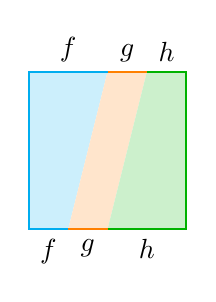
\begin{tikzpicture}
			\path [fill=cyan!20] (0,1)--(-1,1)--(-1,-1)--(-0.5,-1);
			\path [fill=orange!20] (0.5,1)--(0,1)--(-0.5,-1)--(0,-1);
			\path [fill=black!30!green!20] (0.5,1)--(0,-1)--(1,-1)--(1,1);

			\draw [color=cyan, thick] (-0.5,-1)
				-- node [color=black, pos=0.5, below]{$f$} (-1,-1) 
				-- (-1,1)
				-- node [color=black, pos=0.5, above]{$f$} (0,1);

			\draw [color=orange, thick] (-0.5,-1) 
				-- node [color=black, pos=0.5, below]{$g$} (0,-1);
			\draw [color=orange, thick] (0,1) 
				-- node [color=black, pos=0.5, above]{$g$} (0.5,1);

			\draw [color=black!30!green, thick] (0,-1) 
				-- node [color=black, pos=0.5, below]{$h$} (1,-1)
				-- (1,1)
				-- node [color=black, pos=0.5, above]{$h$} (0.5,1);		
		\end{tikzpicture}
	\end{center}
	We can check that $H(s,t)$ is a homotopy rel end points from $h\cdot(g\cdot f)$ to $(h\cdot g)\cdot f$.

	Define a path
	\begin{align*}
		c_x:[0,1] &\longrightarrow X\\
		s &\longmapsto x
	\end{align*}
	We can show that $c_x\cdot f\sim f$ and $f\cdot c_x\sim f$, which means $[c_x]$ is the identity of the group $\pi_1(X,x)$. 

	Given any $[f]\in \pi_1(X,x)$, it is easy to check $\left[f\right]^{-1}\in \pi_1(X,x)$ and $[f]^{-1}\cdot[f]=[f]\cdot[f]^{-1}=[c_x]$.
\end{proof}

\begin{definition}[fundamental groupoid]
	Let $X$ be a topological space. Define $\Pi_1(X)$ to a category, where $\Obj(\Pi_1(X))=X$ and $\Hom_{\Pi_1(X)}(x,y)=\{[f]\mid f:[0,1]\to X \text{ is a path from $x$ to $y$}\}$. $\Pi_1(X)$ is a groupoid and called the fundamental groupoid of $X$.
\end{definition}
\begin{definition}[fundamental groupoid functor]
	Define $\Pi_1:\Top\to\Grpd$ as follows
	\[
	\begin{tikzcd}
		X  \arrow[dd, "f"{name=L, left}] 
		&[-25pt] & [+10pt] 
		& [-30pt] \Pi_1(X) \arrow[dd, "\Pi_1(f)"{name=R}]&[-30pt]\ni
		&[-30pt]\left[p\right]\arrow[dd,mapsto]\\ [-10pt] 
		&  \phantom{.}\arrow[r, "\Pi_1", squigarrow]&\phantom{.}  &   \\[-10pt] 
		Y & & & \Pi_1(Y)&\ni&\left[f\circ p\right]
	\end{tikzcd}
	\]
\end{definition}
\begin{proof}
	First, we will show that $\Pi_1(f)$ is well-defined, namely for any two paths $p_1$ and $p_2$ in $X$,
	\[
		p_1\sim p_2 \implies [f\circ p_1] = [f\circ p_2].
	\]
	Suppose $p_1\sim p_2$ and $h$ is a homotopy rel end points from $p_2$ to $p_2$. Then $r(s,t):=f(h(s, t))$
	is a homotopy rel end points from $f\circ p_1$ to $f\circ p_2$, because for all $s\in[0,1]$,
	\begin{align*}
		r(s,0)&=f(h(s,0))=f(p_1(s))=f\circ p_1(s),\\
		r(s,1)&=f(h(s,1))=f(p_2(s))=f\circ p_2(s).
	\end{align*}
	Thus we have $f\circ p_1\sim f\circ p_2$, which implies $\Pi_1(f)$ is well-defined.
	To verify the functinality of $\Pi_1$, we have to show that
	\[
		\Pi_1(g\circ f) = \Pi_1(g)\circ\Pi_1(f),
	\]
	or equivalently for all $[p]\in \Pi_1(X)$,
	\[
		[(g\circ f)\circ p]=[g\circ (f\circ p)],
	\]
	which clearly holds. 
\end{proof}

\chapter{Covering spaces}
\section{Covering spaces}
\begin{definition}
	Let $X$ be a topological space. A \emph{covering} of $X$ is a continuous map
$$
p: E \rightarrow X
$$
such that there exists a discrete space $D$ and for every $x \in X$ an open neighborhood $U \subset X$, such that $p^{-1}(U)=\bigsqcup_{d \in D} V_d$ and $\left.p\right|_{V_d}: V_d \rightarrow U$ is a homeomorphism for every $d \in D$. Such open neighborhood $U$ is called a \emph{fundamental neighborhood} for $x$. Often, the notion of a covering is used for the covering space $E$ as well as for the map $p: E \rightarrow X$. The open sets $V_d$ are called sheets.
\end{definition}
A covering space is a fiber bundle with discrete fiber $D$, illustrated as follows
\[\xymatrix{
			p^{-1}(U)\ar[rd]_{p}\ar[rr]^{\phi}  & &U\times D\ar[ld]^{p_1}\\
			&U&
			}\]
\begin{proposition}
	The projection $p:E\to X$ is a local homeomorphism.
\end{proposition}
\begin{definition}[lifting]
	Let $p:E\to X$ and $f:Y\to X$ be continuous maps. A lifting of $f$ along $p$ is a continuous map $\tilde{f}:Y\to E$ such that the following diagram commutes
	\[\xymatrix{
			& E\ar[d]^{p}\\
			Y\ar[ur]^{\tilde{f}}\ar[r]_{f} &X
			}\]
\end{definition}
Throughout this chapter, we assume that all given spaces are connected and locally path
connected.

\begin{lemma}
	Let $p: E \rightarrow X$ be a covering. Then the diagonal $D=\{(e, e) \in E \times E \mid e\in E\}$ is open and closed in $Z=\{(e_1, e_2) \in E \times E \mid p(e_1)=p(e_2)\}$.
\end{lemma}
\begin{proof}
	Given any $(e,e)\in D$, suppose $U$ is a fundamental neighborhood of $p(e)$ and $V_e$ is the corresponding sheet such that $\left.p\right|_{V_e}:V_e\to U$ is a homeomorphism. Then for any $e_1,e_2\in V_e$, we have
	\[
		p(e_1)=p(e_2)\implies e_1=e_2,
	\]
	which implies $Z \cap\left(V_e \times V_e\right)=W_e$ is contained in $D$. Note $W_e$ is an open neighbourhood of $(e, e)$ in $Z$. We see $D$ is open in $Z$.

	Given any $(e_1,e_2)\in Z-D$, suppose $U$ is a fundamental neighborhood of $p(e_1)=p(e_2)$ and $V_{e_1}$ and $V_{e_2}$ are the sheets such that $\left.p\right|_{V_{e_1}}:V_{e_1}\to U$, $\left.p\right|_{V_{e_2}}:V_{e_2}\to U$ are a homeomorphisms. Since $e_1 \ne e_2$, we have $V_{e_1} \cap V_{e_2}=\varnothing$ and $\left(V_{e_1}\times V_{e_2}\right)\cap D=\varnothing$. Hence $Z \cap\left(V_{e_1} \times V_{e_2} \right)$  is contained in $Z-D$. Note that $Z \cap\left(V_{e_1} \times V_{e_2} \right)$ is an open neighbourhood of $(e_1,e_2)$ in $Z$. This shows that $Z- D$ is also open.
\end{proof}

\begin{proposition}[uniqueness of liftings]
Let $p: E \rightarrow X$ be a covering. Let $\tilde{f}_1, \tilde{f}_2: Y \rightarrow E$ be liftings of $f: Y \rightarrow X$. Suppose $\tilde{f}_1(y_0)=\tilde{f}_2(y_0)$ for some $y_0\in Y$. If $Y$ is connected, then $\tilde{f}_1=\tilde{f}_2$.
\end{proposition}
\begin{proof}
	Suppose $Z=\{(e_1, e_2) \in E \times E \mid p(e_1)=p(e_2)\}$ and $D=\{(e, e) \in E \times E \mid e\in E\}$. We can define a continuous map
	\begin{align*}
		g: Y &\longrightarrow Z\\
		y &\longmapsto \left(\tilde{f}_1(y), \tilde{f}_2(y)\right)
	\end{align*}
	 By assumption, $g(y_0)\in D$, which guarantees $g^{-1}(D)$ is nonempty. By lemma 4.1.1, we see $g^{-1}(D)$ is open and closed in $Y$. If $Y$ is connected, then $g^{-1}(D)=Y\implies g(Y)\subseteq D$. In other words, we have
	 \[
		\left\{\left(\tilde{f}_1(y), \tilde{f}_2(y)\right) \midv y \in Y\right\} \subseteq\{(e, e) \in E \times E \mid e\in E\}.
		\]
	Therefore, we show that	$\tilde{f}_1=\tilde{f}_2$.
\end{proof}

\begin{proposition}[path lifting]
	Let $p: E \to X$ be a covering, let $x \in X$, and let $e, e^{\prime}$ be any two points in $p^{-1}(x)$. A path $f: I \to B$ with $f(0)=x$ lifts uniquely to a path $\tilde{f}: I \to E$ such that $\tilde{f}(0)=e$ and $p \circ \tilde{f}=f$.
\end{proposition}
\begin{proof}
	Suppose $\mathcal{F}=\left\{U_\alpha\right\}_{\alpha\in A}$ is a collection of fundamental neighborhoods such that $\cup_{\alpha\in A}U_\alpha=X$. Let $f:I\to X$ be a path with $f(0)=x$. Then $\left\{f^{-1}(U_\alpha)\right\}_{\alpha\in A}$ is an open cover of $I$, so has a finite subcover $\left\{f^{-1}(U_{i})\right\}_{i=1}^m$. Let $0=t_0<t_1<\cdots<t_n=1$ be such that $f([t_{k-1},t_k])\subseteq U_{i_k}$ where $1\le i_k \le m$. \\
	We will construct a sequence of maps $\tilde{f}_k:[t_{k-1},t_k]\to E$ by induction on $k$. Suppose $k=0$. Note that $f(0)=x\in U_{i_0}$ and there exists a homeomorphism $\left.p\right|_{V_0}: E\supseteq V_0\to U_{i_0}$ such that $\left.p\right|_{V_0}(e)=x$. We can define $\tilde{f}_0=\left(\left.p\right|_{V_0}\right)^{-1}\circ f|_{[t_0,t_1]}$ and check that $\tilde{f}_0$ is a lifting of $f|_{[t_0,t_1]}$ such that $\tilde{f}_0(0)=e$. \\
	Suppose we have constructed $\tilde{f}_0,\tilde{f}_1,\cdots,\tilde{f}_{k-1}$. Note that $f(t_{k})=p\left(\tilde{f}_{k-1}(t_k)\right)\in U_{i_k}$ and there exists a homeomorphism $\left.p\right|_{V_k}: E\supseteq V_k\to U_{i_k}$ such that $\left.p\right|_{V_{k}}\left(\tilde{f}_{k-1}(t_k)\right)=f(t_k)$. We can define $\tilde{f}_k=\left(\left.p\right|_{V_k}\right)^{-1}\circ f|_{[t_k,t_{k+1}]}$ and check that $\tilde{f}_k$ is a lifting of $f|_{[t_k,t_{k+1}]}$ such that $\tilde{f}_k(t_{k})=\tilde{f}_{k-1}(t_{k})$. \\
	By defining 
	\[
		\tilde{f}(t)=\tilde{f}_k(t)\text{ for }t_{k}\le t\le t_{k+1},	
	\]
	we can connect the sequence of maps $\tilde{f}_k$ to get a path $\tilde{f}:I\to E$ such that $\tilde{f}(0)=e$ and $p\circ \tilde{f}=f$. Since $I$ is connected, we know $\tilde{f}$ is unique.
\end{proof}

\begin{proposition}[unique path lifting]
	Let $p: E \to X$ be a covering, let $x \in X$, and let $e, e^{\prime}$ be any two points in $p^{-1}(x)$.
	\begin{enumerate}[(i)]
		\item A path $f: I \to B$ with $f(0)=x$ lifts uniquely to a path $\tilde{f}: I \to E$ such that $\tilde{f}(0)=e$ and $p \circ \tilde{f}=f$.
		\item Equivalent paths $f_1 \sim f_2: I \to X$ that start at $x$ lift to equivalent paths $\tilde{f}_1\sim \tilde{f}_2: I \to E$ that start at $e$, hence $\tilde{f}_1(1)=\tilde{f}_2(1)$, i.e $\tilde{f}_1$ and $\tilde{f}_2$ end at the same point in $E$.
		\item $p_*: \pi_1(E, e) \to \pi_1(B, b)$ is a monomorphism.
		\item $p_*\left(\pi_1\left(E, e^{\prime}\right)\right)$ is conjugate to $p_*\left(\pi_1(E, e)\right)$.
		\item As e' runs through $F_b$, the groups $p_*\left(\pi_1\left(E, e^{\prime}\right)\right)$ run through all conjugates of $p_*\left(\pi_1(E, e)\right)$ in $\pi_1(B, b)$.
	\end{enumerate}
\end{proposition}
\begin{proof}
\end{proof}
\chapter{Homology}
\section{Simplicial homology}

\begin{definition}[geometrically independent]
	Let $\left\{a_0, a_1, \cdots, a_k\right\}$ be points in $\mathbb{R}^n$. This set is said to be \emph{geometrically independent} if the vectors
$$
a_1-a_0, \quad a_2-a_0, \quad \cdots, \quad a_k-a_0
$$
are linearly independent (as in linear algebra).
\end{definition}

\begin{definition}[simplex]
Let $\left\{a_0, a_1, \ldots, a_k\right\}$ be a geometrically independent set in $\mathbb{R}^n$. A $\emph{$k$-simplex } \sigma$ spanned by these points is defined by
$$
\left\{x\in \mathbb{R}^n\;\left|\; x=\sum_{i=0}^k t_i a_i,\;\sum_{i=0}^k t_i=1,\;t_i \geq 0\text{ for }i = 0,1,\cdots, k\right.\right\}.
$$
\end{definition}

\noindent A $k$-simplex spanned by $a_0, a_1, \ldots, a_k$ is the convex hull of these points.
\begin{definition}
Let $\sigma$ be a $k$-simplex spanned by $\left\{a_0, a_1, \ldots, a_k\right\}$.
\begin{enumerate}
	\item The points $a_0, a_1, \ldots, a_k$ are called the \emph{vertices} of $\sigma$.
	\item The number $k$ is the \emph{dimension} of $\sigma$.
	\item Any simplex spanned by a subset of $\left\{a_0, a_1, \cdots, a_k\right\}$ is called a \emph{face} of $\sigma$. 
	\item The face spanned by $\left\{a_0, a_1, \cdots, a_k\right\}-\left\{a_i\right\}$ for some $i$ is called the \emph{face opposite} to $a_i$.
	\item A face of $\sigma$ is called a \emph{proper face} if it is not equal to $\sigma$.
	\item The union of all proper faces of $\sigma$ is called the \emph{boundary} of $\sigma$, denoted by $\partial \sigma$.
	\item $\sigma-\partial \sigma$ is called the \emph{interior} of $\sigma$.
\end{enumerate}
\end{definition}
\begin{definition}[simplicial complex]
A \emph{simplicial complex} $K$ is a collection of simplices in $\mathbb{R}^n$ (of possibly varying dimensions) such that
\begin{enumerate}
	\item Any face of a simplex in $K$ is also in $K$.
	\item The intersection of any two simplices in $K$ is a face of each of the two simplices, whenever the the intersection is non-empty.
\end{enumerate}
\end{definition}

\begin{definition}[subcomplex]
Let $K$ be a simplicial complex. If $L\subset K$ and $L$ is a simplicial complex, then $L$ is called a \emph{subcomplex} of $K$.
\end{definition}

\begin{definition}[$p$-skeleton]
Given a simplicial complex $K$, the collection of all simplices of $K$ of dimension at $\operatorname{most} p$ is called the $\emph{$p$-skeleton}$ of $K$ and is denoted $K^{(p)}$.
\end{definition}
For example, $K^{(0)}$ is the set of vertices of $K$. $K^{(p)}$ is a subcomplex of $K$.

\begin{definition}[dimension of a simplicial complex]
If there exists an integer $N$ such that
$$
K^{(N-1)} \neq K \quad \text { and } \quad K^{(p)}=K \text { for }p\ge N ,
$$
then $K$ is said to have \emph{dimension} $N$. Otherwise it is said to have infinite dimension.
\end{definition}
\begin{definition}[finite simplicial complex]
A simplicial complex $K$ is said to be \emph{finite} if $K^{(0)}$ is finite.
\end{definition}

\begin{definition}[realization of a simplicial complex]
The realization of a simplicial complex $K$ is a topological space $(|K|, \tau)$ such that
\begin{enumerate}
	\item $|K|$ is the union of all simplices in $K$, that is $|K|=\bigcup_{\sigma\in K}\sigma$.
	\item $F\subset |K|$ is a closed set in $(|K|, \tau)\iff$ for all simplices $\sigma\in K$, $F\cap \sigma$ is a closed set in $(\sigma,\nu_\sigma)$, where $\nu_\sigma$ is the subspace topology of Euclidean topology.
\end{enumerate}
\end{definition}
For finite simplicial complexes $K$ with finite dimension, the topology $\tau$ coincides with the subspace topology of Euclidean topology. 
\begin{definition}[triangulation]
	A \emph{triangulation} of a topological space $X$ is a simplicial complex $K$ together with a homeomorphism $\phi:|K|\to X$.
\end{definition}
All smooth manifolds are triangulable. For example, torus admits the following triangulation:
\begin{center}
	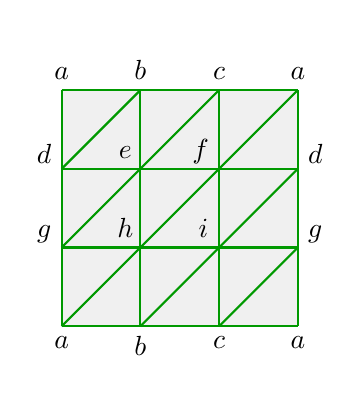
\begin{tikzpicture}[add_padding, x=1.5cm,y=1.5cm]
		\fill[fill=gray!12] (-1,-1)--(1,-1)--(1,1)--(-1,1)-- cycle;
		\draw [color=black!40!green,thick] (-1,-1) --
		node [color=black,pos=0,below]{$a$}
		node [color=black,pos=1/3,below]{$b$}
		node [color=black,pos=2/3,below]{$c$}
		node [color=black,pos=1,below]{$a$}(1,-1);
		\draw [color=black!40!green,thick] (-1,1/3)--		
		node [color=black,pos=0.27,above]{$e$} 
		 (1,1/3);
		\draw [color=black!40!green,thick] (-1,-1/3)--
		node [color=black,pos=0.27,above]{$h$} 
		node [color=black,pos=0.60,above]{$i$} (1,-1/3);
		\draw [color=black!40!green,thick] (-1/3,-1)--(-1/3,1);
		\draw [color=black!40!green,thick] (1/3,-1)--node [color=black,pos=0.74,left]{$f$}(1/3,1);
		\draw [color=black!40!green,thick] (1/3,-1)--(1,-1/3);
		\draw [color=black!40!green,thick] (-1/3,-1)--(1,1/3);
		\draw [color=black!40!green,thick] (-1,-1)--(1,1);
		\draw [color=black!40!green,thick] (-1,-1/3)--(1/3,1);
		\draw [color=black!40!green,thick] (-1,1/3)--(-1/3,1);
		\draw [color=black!40!green,thick] (-1,1)--
		node [color=black,pos=0.27,left]{$d$} 
		node [color=black,pos=0.61,left]{$g$} (-1,-1);
		\draw [color=black!40!green,thick] (1,1)--
		node [color=black,pos=0.27,right]{$d$} 
		node [color=black,pos=0.61,right]{$g$} (1,-1);
		\draw [color=black!40!green,thick] (-1,1)-- 
		node [color=black,pos=0,above]{$a$} 
		node [color=black,pos=1/3,above]{$b$} 
		node [color=black,pos=2/3,above]{$c$}
		node [color=black,pos=1,above]{$a$} 
		(1,1);
	\end{tikzpicture}
\end{center}

\begin{definition}[orientation of simplex]
	Suppose $\sigma$ is a $k$-simplex spanned by $\left\{a_0, a_1, \ldots, a_k\right\}$. Let $V_{\sigma}$ to be the set of all ordered $k+1$-tuples of vertices of $\sigma$:
	\begin{align*}
		V_{\sigma}=\left\{\left(a_{s(0)},a_{s(1)},\cdots,a_{s(k)}\right)\mid s\in \mathrm{Sym}\left(\left\{0,1,\cdots,k\right\}\right)\right\}.
	\end{align*}
	Then $\sim$ is an equivalence relation on $V_{\sigma}$, where $\sim$ is defined by
	\begin{align*}
		\left(a_{s(0)},\cdots,a_{s(k)}\right)\sim\left(a_{s'(0)},\cdots,a_{s'(k)}\right)\iff \mathrm{sgn}(s)=\mathrm{sgn}(s').
	\end{align*}
	An orientation of $\sigma$ is a equivalence class of $V_{\sigma}/\sim$, denoted by
	\begin{align*}
		\left[a_{s(0)},a_{s(1)},\cdots,a_{s(k)}\right].
	\end{align*}
\end{definition}
Every $k$-simplex has exactly $2$ orientations.
\begin{definition}[oriented simplex]
	Let $\sigma$ be a $k$-simplex spanned by $\left\{a_0, a_1, \ldots, a_k\right\}$. An \emph{oriented $k$-simplex} is a pair $\left(\sigma, \left[a_{s(0)},a_{s(1)},\cdots,a_{s(k)}\right]\right)$, where $\sigma$ is a $k$-simplex and $\left[a_{s(0)},a_{s(1)},\cdots,a_{s(k)}\right]$ is an orientation of $\sigma$. The oriented $k$-simplex can be denoted by $\left\langle a_{s(0)},a_{s(1)},\cdots,a_{s(k)}\right\rangle$.
\end{definition}

\begin{definition}[simplicial chain group]
	Let $K$ be a simplicial complex and $F(K)$ be the free abelian group generated by all the oriented $k$-simplices in $K$. The $k$\emph{-chain group} of $K$, denoted by $C_k(K)$, is defined as $F(K)$ modulo the relations
	\begin{align*}
		\left\langle a_{0}, \cdots ,a_{i},\cdots,a_{j},\cdots a_{k}\right\rangle=-\left\langle a_{0},\cdots ,a_{j},\cdots,a_{i},\cdots,a_{k}\right\rangle.
	\end{align*}
\end{definition}
$C_k(K)$ is a free abelian group.
\begin{definition}[boundary homomorphism]
	Given a simplicial complex $K$, we can define the boundary homomorphism $\partial_k:C_k(K)\rightarrow C_{k-1}(K)$ on the basis of $C_k(K)$ by
	\begin{align*}
		\partial_k\left\langle a_{0},a_{1},\cdots,a_{k}\right\rangle=\sum_{i=0}^k(-1)^{i}\left\langle a_{0},a_{1},\cdots,a_{i-1},a_{i+1},\cdots,a_{k}\right\rangle,
	\end{align*}
	and then extend it to the whole $C_k(K)$ linearly.
\end{definition}

\begin{definition}[cycle group]
	Let $K$ be a simplicial complex. The $k$-cycle group of $K$, denoted by $Z_k(K)$,  is defined as $\ker\partial_k$.
\end{definition}

\begin{definition}[boundary group]
	Let $K$ be a simplicial complex. The $k$-boundary group of $K$, denoted by $B_k(K)$, is defined as $\mathrm{im}\,\partial_{k+1}$.
\end{definition}

\begin{proposition}[chain complex]
	Let $K$ be a simplicial complex. Then we have $\partial_k\circ\partial_{k+1}=0$ or equivalently $B_k(K)\subset Z_k(K)$. Therefore we have a chain complex 
	\begin{align*}
		\cdots\stackrel{\partial_{k+2}}{\longrightarrow}  C_{k+1}(K)\stackrel{\partial_{k+1}}{\longrightarrow} C_{k}(K)\stackrel{\partial_{k}}{\longrightarrow} \cdots\stackrel{\partial_{2}}{\longrightarrow}  C_1(K)\stackrel{\partial_{1}}{\longrightarrow} C_0(K)\stackrel{\partial_{0}}{\longrightarrow}  0
	\end{align*}
	in $\mathsf{Ch}(\mathsf{Ab})$. 
\end{proposition}

\begin{definition}[simplical homology group]
	For a simplicial complex $K$, the $k$-th homology group, $H_k(K)$ is defined to be the quotient group $Z_k(K) / B_k(K)$. An element of $H_k(K)$ is called a $k$-dimensional homology class of $K$. We say cycles $z_1, z_2\in Z_k(K)$ are homologous, written as $z_1\sim z_2$, if $z_1-z_2 \in B_k(K)$. 
\end{definition}

\section{Singular homology}
\begin{definition}[standard simplex]
	For $n \geq 0$, the \emph{standard $n$-simplex} $\Delta^n$ is the set $\Delta^n \subset \mathbb{R}^{n+1}$ defined by
$$
\Delta^n=\left\{\left(t_0, \cdots, t_n\right) \in \mathbb{R}^{n+1}\,\middle\vert\, \sum_{i=0}^n t_i=1, t_i \geq 0 \text { for all } i\right\} .
$$
Assume that $(e_0,\cdots,e_n)$ is the standand orthonormal basis of $\mathbb{R}^{n+1}$. Another way to describe $\Delta^n$ is to say that it is the $n$-simplex with vertices $\{e_0,\cdots,e_n\}$.
\end{definition}
\begin{definition}[singular simplex]
	Let $X$ be a topological space. A \emph{singular $n$-simplex} in $X$ is a continuous map $\sigma: \Delta^n \rightarrow X$. All the singular simplices in $X$ constitute $\mathrm{Hom}_{\mathsf{Top}}\left(\Delta^n, X\right)$.
\end{definition}
\begin{definition}[singular chain group functor $C_k$]
	Given a topological space $X$, the \emph{singular $k$-chain group} $C_k(X)$ of $X$ is the free abelian group generated by the singular simplices in $X$. \\
	The singular chain group functor $C_k:\mathsf{Top}\to\mathsf{Ab}$ can be defined as the composition of hom functor and free functor
	\begin{align*}
		\mathsf{Top}\xrightarrow{\mathrm{Hom}_{\mathsf{Top}}\left(\Delta^k, -\right)} \mathsf{Set}\xrightarrow{\mathbb{Z}^\oplus} \mathsf{Ab}
	\end{align*}
	We can also write it explicily as
	\begin{equation*}
		\begin{tikzcd}
			X  \arrow[dd, "f"{name=L, left}] &[-25pt] & [+10pt] & [-30pt] C_k(X) \arrow[dd, "f_\sharp"{name=R}]&[-30pt]\ni&[-30pt]\sigma\arrow[dd,mapsto]\\ [-10pt] 
			                                &  \phantom{.}\arrow[r, "C_k", squigarrow]&\phantom{.}  &   \\[-10pt] 
			Y & & & C_k(Y)&\ni&f\circ \sigma
		\end{tikzcd}
	\end{equation*}
\end{definition}

\begin{definition}[face inclusion]
	For any $k\ge 0$, we can define the \emph{$i$-th face inclusion} by
	\begin{align*}
		l_i: \Delta^{k} &\longrightarrow  \Delta^{k+1}\\
		(t_0, \cdots, t_k) &\longmapsto (t_0, \cdots, t_{i-1}, 0, t_{i}, \cdots, t_{k})
	\end{align*}
	for $0\leq i\leq k+1$. 
\end{definition}
Suppose $\{e_0,\cdots,e_{k+1}\}$ is the vertices of $\Delta^{k+1}$. $l_i$ embeds the face opposite to $e_i$ into $\Delta^{k+1}$.

\begin{proposition}
	If $k\ge 2$, the following diagram commutes:
	\begin{equation*}
		\begin{tikzcd}
			\Delta^{k-2} \arrow[r, "l_i"] \arrow[d, "l_{j-1}"']
			& \Delta^{k-1}  \arrow[d, "l_{j}"] \\ [5pt]
			\Delta^{k-1}  \arrow[r, "l_i"']
			&  \Delta^{k} 
		\end{tikzcd}			
	\end{equation*}
	for $0\le i\le j-1\le k-1$. That is, $l_j\circ l_i=l_i\circ l_{j-1}$.
\end{proposition}
\begin{proof}
	If $i<j-1$, then
	\[
	\begin{aligned}
		\left(l_i\circ l_{j-1}\right)(t_0, \cdots, t_{k-2})&=l_i\left(l_{j-1}(t_0, \cdots, t_{k-2})\right)\\
		&=l_i\left(t_0, \cdots, t_{j-2}, 0, t_{j-1}, \cdots, t_{k-2}\right)\\
		&=\left(t_0, t_{i-1},0,t_{i},\cdots, t_{j-2}, 0, t_{j-1}, \cdots, t_{k-2}\right)\\
		&=l_j\left(t_0, \cdots, t_{i-1}, 0, t_{i}, \cdots, t_{k-2}\right)\\
		&=l_j\left(l_i(t_0, \cdots, t_{k-2})\right)\\
		&=(l_j \circ l_i)(t_0, \cdots, t_{k-2}).
	\end{aligned}
	\]
\end{proof}

\begin{definition}[boundary homomorphism]
	Given a topological space $X$, we can define the boundary map $\partial_k:C_k(X)\rightarrow C_{k-1}(X)$ on $\sigma:\Delta^k\to X$ by
	\begin{align*}
		\partial_k\left(\sigma\right)=\sum_{i=0}^k(-1)^{i}\sigma\circ l_i,
	\end{align*}
	and then extend it to the whole $C_k(X)$ linearly.
\end{definition}

\begin{definition}[singular cycle group]
	Let $X$ be a topological. The $k$-cycle group of $K$, denoted by $Z_k(X)$,  is defined as $\ker\partial_k$.
\end{definition}

\begin{definition}[singular boundary group]
	Let $X$ be a topological. The $k$-boundary group of $K$, denoted by $B_k(X)$, is defined as $\mathrm{im}\,\partial_{k+1}$.
\end{definition}

\begin{proposition}
	Let $X$ be a topological space. Then we have $B_k(X)\subset Z_k(X)$ or equivalently $\partial_k\circ\partial_{k+1}=0$.
\end{proposition}
\begin{proof}
	\[
	\begin{aligned}
		\left(\partial_k\circ\partial_{k+1}\right)(\sigma)&=\partial_{k}\circ\left(\sum_{j=0}^{k+1}(-1)^{j}\sigma\circ l_j\right)\\
		&=\sum_{j=0}^{k+1}(-1)^{j}\partial_{k}\circ\sigma\circ l_j\\
		&=\sum_{j=0}^{k+1}(-1)^{j}\left(\sum_{i=0}^k(-1)^{i}\sigma\circ l_j\circ l_i\right)\\
		&=\sum_{i=0}^{k}\sum_{j=0}^{k+1}(-1)^{i+j}\sigma\circ l_j\circ l_i\\
		&=\sum_{0\le i\le j-1\le k}(-1)^{i+j}\sigma\circ l_j\circ l_i+\sum_{0\le j\le i\le k}(-1)^{i+j}(-1)^{i+j}\sigma\circ l_j\circ l_i\\
		&=\sum_{0\le i\le j-1\le k}(-1)^{i+j}\sigma\circ l_i\circ l_{j-1}+\sum_{0\le j\le i\le k}(-1)^{i+j}\sigma\circ l_j\circ l_i\\
		&=\sum_{0\le i\le m\le k}(-1)^{i+m+1}\sigma\circ l_i\circ l_{m}+\sum_{0\le j\le i\le k}(-1)^{i+j}\sigma\circ l_j\circ l_i\\
		&=-\sum_{0\le j\le i\le k}(-1)^{i+j}\sigma\circ l_j\circ l_{i}+\sum_{0\le j\le i\le k}(-1)^{i+j}\sigma\circ l_j\circ l_i\\
		&=0.
	\end{aligned}
	\]
\end{proof}

\begin{definition}[singular chain complex functor $C_.$]
	 We have a chain complex $C_{\boldsymbol{\cdot}}(X)$
	\begin{align*}
		\cdots\stackrel{\partial_{k+2}}{\longrightarrow}  C_{k+1}(X)\stackrel{\partial_{k+1}}{\longrightarrow} C_{k}(X)\stackrel{\partial_{k}}{\longrightarrow} \cdots\stackrel{\partial_{2}}{\longrightarrow}  C_1(X)\stackrel{\partial_{1}}{\longrightarrow} C_0(X)\stackrel{\partial_{0}}{\longrightarrow}  0
	\end{align*}
	in $\mathsf{Ch}(\mathsf{Ab})$. The singular chain complex functor $C_{\boldsymbol{\cdot}}:\mathsf{Top}\to\mathsf{Ch}(\mathsf{Ab})$ is defined as follows:
	\begin{equation*}
		\begin{tikzcd}
			X  \arrow[dd, "f"{name=L, left}] &[-25pt] & [+10pt] & [-30pt] C_{\boldsymbol{\cdot}}(X) \arrow[dd, "f_\sharp"{name=R}]\\ [-10pt] 
			                                &  \phantom{.}\arrow[r, "C_{\boldsymbol{\cdot}}", squigarrow]&\phantom{.}  &   \\[-10pt] 
			Y & & & C_{\boldsymbol{\cdot}}(Y)
		\end{tikzcd}
	\end{equation*}
\end{definition}
\begin{proof}
	To show that $C_{\boldsymbol{\cdot}}$ is a functor, we need to check that the following diagram commutes
	\begin{equation*}
		\begin{tikzcd}
			C_{k}(X) \arrow[r, "\partial_{k}"] \arrow[d, "f_\sharp"']
			& C_{k-1}(X) \arrow[d, "f_\sharp"] \\ [5pt]
			C_{k}(Y) \arrow[r, "\partial_{k}"']
			&  C_{k-1}(Y) 
		\end{tikzcd}			
	\end{equation*}
	That is,
	\[
	\begin{aligned}
		(\partial_k\circ f_\sharp)(\sigma)&=\partial_k\left(f_\sharp(\sigma)\right)\\
		&=\partial_k\left(f\circ\sigma\right)\\
		&=\sum_{i=0}^k(-1)^{i}f\circ\sigma\circ l_i\\
		&=\sum_{i=0}^k(-1)^{i}f_\sharp\left(\sigma\circ l_i\right)\\
		&=f_\sharp\left(\sum_{i=0}^k(-1)^{i}\sigma\circ l_i\right)\\
		&=f_\sharp(\partial_k(\sigma))\\
		&=(f_\sharp\circ\partial_k)(\sigma).
	\end{aligned}
	\]
\end{proof}

\begin{definition}[singular homology group functor $H_k$]
	Given a topological space $X$, the \emph{$k$-th homology group} $H_k(X)$ is defined to be the quotient group $Z_k(X) / B_k(X)$. \\
	The $k$-th singular homology group functor $H_k:\mathsf{Top}\to\mathsf{Ab}$ is the composition of the singular complex functor with the homology functor
	\begin{align*}
		\mathsf{Top}\xrightarrow{C_{\boldsymbol{\cdot}}} \mathsf{Ch}(\mathsf{Ab})\xrightarrow{H_k'} \mathsf{Ab}
	\end{align*}
	which can be written explicitly as follows
	\begin{equation*}
		\begin{tikzcd}
			X  \arrow[dd, "f"{name=L, left}] &[-25pt] & [+10pt] & [-30pt] H_k(X) \arrow[dd, "f_*"{name=R}]&[-30pt]\ni&[-30pt]\sigma +B_k(X)\arrow[dd,mapsto]\\ [-10pt] 
			&  \phantom{.}\arrow[r, "H_k", squigarrow]&\phantom{.}  &   \\[-10pt] 
			Y & & & H_k(Y)&\ni&f\circ \sigma+B_k(Y)
		\end{tikzcd}
	\end{equation*}
\end{definition}

\begin{proposition}
For any topological space $X$, we have a natural isomorphism 
$$
H_k(X)\cong\bigoplus_{\alpha\in \pi_0(X)} H_k\left(X_\alpha\right),
$$ 
where $X_\alpha$ are path-components of $X$. Especially, we have $H_0(X)\cong \mathbb{Z}^{\oplus \pi_0(X)}$. 
\end{proposition}
\begin{proof}
	First we apply the functor $C_k:\mathsf{Top}\to\mathsf{Ab}$ to the inclusions $i_\alpha:X_\alpha \hookrightarrow X$ to get $\left(i_\alpha\right)_\sharp$
	\begin{align*}
		\left(i_\alpha\right)_\sharp: C_k(X_\alpha)&\longrightarrow C_k(X)\\
                   \sigma &\longmapsto i_\alpha\circ \sigma
	\end{align*}
	Then the unversal property of copruduct gives a unique homomorphism $\varphi$ such that the following diagram commutes
	\begin{equation*}
		\begin{tikzcd}		
			& C_{k}(X) \\ [10pt]
			C_{k}(X_\alpha) \arrow[ru, "\left(i_\alpha \right)_{\sharp}"] \arrow[r, "j_\alpha"']
			& \bigoplus\limits_{\alpha\in \pi_0(X)} C_k\left(X_\alpha\right) \arrow[u, "\varphi"'] 
		\end{tikzcd}			
	\end{equation*}
	The commutative diagram implies that given a map $\sigma_\alpha:\Delta^k\to X_\alpha$ in $C_k(X_\alpha)$, we have
	\[
		\varphi(\sigma_\alpha)=\varphi(j_\alpha(\sigma_\alpha))=\left(i_\alpha\right)_\sharp(\sigma_\alpha)=i_\alpha\circ\sigma_\alpha.
	\]
	$\bigoplus\limits_{\alpha\in \pi_0(X)} C_k\left(X_\alpha\right)$ as a direct sum of free abelian groups is free, and its basis is the union of the basis of each $C_k\left(X_\alpha\right)$. 
	For any $\sum\limits_{\alpha\in J}c_\alpha\sigma_\alpha\in \bigoplus\limits_{\alpha\in \pi_0(X)} C_k\left(X_\alpha\right)$, where $\sigma_\alpha\in C_k\left(X_\alpha\right)$ are distinct maps, we have
	\[
		\varphi\left(\sum\limits_{\alpha\in J}c_\alpha\sigma_\alpha\right)=0\implies \sum_{\alpha\in J}c_\alpha\varphi\left(\sigma_\alpha\right)=\sum_{\alpha\in J} c_\alpha \left(i_\alpha\circ\sigma_\alpha\right)=0\implies \forall \alpha\in J,\;c_\alpha=0,
	\]
	which implies $\varphi$ is a monomorphism. 

	For any map $\sigma:\Delta^k\to X$ in $C_k(X)$, since $\Delta^k$ is path-connected, there must be $\sigma(\Delta^k)\subset X_\alpha$, where $X_\alpha$ is a path-component of $X$. Let $\sigma_\alpha:\Delta^k\to X_\alpha$, $x\mapsto\sigma(x)$. Then we have $\varphi(\sigma_\alpha)=i_\alpha\circ\sigma_\alpha=\sigma$, which implies $\varphi$ is an epimorphism. Therefore, $\varphi$ is an isomorphism. Since functor $H_k'$ preserves isomorphism, we obtain
	$$
	H_k(X)=H_k'(C_k(X))\cong H_k'\left(\bigoplus_{\alpha\in \pi_0(X)} C_k\left(X_\alpha\right)\right).
	$$ 
	In general, for any AB5 category $\mathsf{A}$, the homology functor $H_k:C_\text{\hspace{-1pt}\huge$.$\hspace{-1pt}}(\mathsf{A})\to \mathsf{A}$ preserves coproduct. In particular, $\mathsf{Ab}$ is an AB5 category. Therefore, we completes the proof.
\end{proof}

\begin{proposition}[homotopy induces chain homotopy]
	If two maps $f,g :X\to Y$ are homotopic, then there exists a chain homotopy between $f_\sharp$ and $g_\sharp$.
\end{proposition}
\begin{proof}
	Suppose $I=[0,1]$ and
	\begin{align*}
		i_0: X &\longrightarrow X\times I\\
		p&\longmapsto (p,0)
	\end{align*}
	\begin{align*}
		i_1: X &\longrightarrow X\times I\\
		p&\longmapsto (p,1)
	\end{align*}
	We first show this proposition for $Y=I$ and $f=i_0$, $g=i_1$. 
	
	
	Now let's consider the general case. Assume $h$ is a homotopy between $f\overset{h}{\sim} g$. Then we have $f=h\circ i_0$ and $g=h\circ i_1$
	
	\begin{equation*}
		\begin{tikzcd}		
			X \arrow[r, shift left=1.2, "i_0"]\arrow[r,shift right=1.2,"i_1"']  \arrow[rr, bend left=42, "f"{ above}] \arrow[rr, bend right=42, "g"{below}]
			& X\times I \arrow[r, "h"] & Y
		\end{tikzcd}			
	\end{equation*}
	\[
	\begin{aligned}
		g-f &= h\circ i_1 - h\circ i_0\\
		&= h\circ (i_1-i_0)\\
		&= 1
	\end{aligned}
	\]
\end{proof}

\begin{proposition}[homotopy invariance of singular homology]
	If two maps $f,g :X\to Y$ are homotopic, then we have $H_k(f)=H_k(g)$, or equivalently, $f_*\cong g_*$.
\end{proposition}

\section{Axiomatic homology theory}
\begin{definition}[the category of pairs of topological spaces $\mathsf{Top}_{(2)}$]
	The object of $\mathsf{Top}_{(2)}$ are pairs $(X, A)$ of topological spaces, where $A$ is a subspace of $X$. The morphisms between $(X, A)$ and $(Y, B)$ are continuous maps $f:X\to Y$ such that $f(A)\subset B$.
\end{definition}

\begin{definition}[the functor $K$]
	functor $K:\mathsf{Top}_{(2)}\to\mathsf{Top}_{(2)}$ is defined as follows:
	\begin{equation*}
		\begin{tikzcd}
			(X,A)  \arrow[dd, "f"{name=L, left}] &[-25pt] & [+10pt] & [-30pt] (A, \varnothing) \arrow[dd, "\left.f\right|_A"{name=R}]\\ [-10pt] 
			                                &  \phantom{.}\arrow[r, "K", squigarrow]&\phantom{.}  &   \\[-10pt] 
			(Y,B) & & & (B, \varnothing)
		\end{tikzcd}
	\end{equation*}
\end{definition}

\begin{definition}[Eilenberg–Steenrod axioms]
	A homology theory on a topological space refers to the following data that satisfies the given axioms:
	\begin{itemize}
		\item Functors $H_n:\mathsf{Top}_{(2)}\to \mathsf{Ab}$, $n\in\mathbb{Z}$,
		\item Natural transformations $\partial_n:H_n\to H_{n-1}\circ K$, $n\in\mathbb{Z}$,
	\end{itemize}
	The axioms are:
	\begin{itemize}
		\item Homotopy: If $f:(X, A)\to (Y, B)$ is homotopic to $g:(X, A)\to (Y, B)$, then $H_n(f)=H_n(g)$ for all $n\in\mathbb{Z}$.
		\item Excision: For any pair $(X, A)$, if $U$ is a subset of $A$ such that $\overline{U}\subset X^\circ$, then $$H_n(X,A)\cong H_n(X-U,A-U)$$
		for all $n\in\mathbb{Z}$.
		\item Dimension: Let $\left\{*\right\}$ be a one-point space. Then $H_n(\left\{*\right\}) = 0$ for all $n \neq 0$. Here $H_n(\left\{*\right\})$ is a shorthand for $H_n(\left\{*\right\}, \varnothing)$.
		\item Additivity:
		\[
H_n\left(\coprod_{\alpha\in I} X\right)\cong\bigoplus_{\alpha\in I} H_n\left(X_\alpha\right).
			\]
		\item Exactness: Each pair $(X,A)$ induces along exact sequenceinhomology, via the inclusions $i: A\hookrightarrow X$ and $j:X\hookrightarrow (X, A)$ 
		$$
		\cdots \to H_n(A) \,\xrightarrow{i_*}\, H_n(X) \,\xrightarrow{j_*}\, H_n (X,A) \,\xrightarrow{\partial}\, H_{n-1}(A) \to \cdots
		$$
	\end{itemize}
\end{definition}



\chapter{Concrete Examples}
A topological space $X$ is called locally Euclidean if there is a non-negative integer $n$ such that every point in $X$ has a neighbourhood which is homeomorphic to real n-dimensional space $\mathbb{R}^n$.

\indent A topological manifold is a locally Euclidean Hausdorff space. In this chapter we focus on some concrete topological manifolds to develop a topological intuition. Topological manifold will be called manifold in brief whenever we mention it.

\section{One-dimensional manifolds}
\subsection{Real affine line $\mathbb{R}^1$}
The real line $\mathbb{R}^1$ carries a standard topology, which can be introduced from the metric defined above. The real line is homeomorphic to any open interval $(a, b)\in\mathbb{R}$.
\begin{center}
	\begin{tikzpicture}
		\path (-4,0.5) node (name1) {$\mathbb{R}^1$};
		\path (4,0.5) node (name2) {$(a,b)$};
		\draw (-6,0) -- (-2,0);
		\draw (name1);
		\draw (0,0) node {$\cong$};
		\draw (2,0) circle [radius=2pt] (2.05,0)-- (5.95,0)(6,0) circle [radius=2pt];
		\draw (name2);
	\end{tikzpicture}
\end{center}
One homeomorphic mapping is
\begin{align*}
	f:\mathbb{R}^1\longrightarrow(a, b),\qquad
	x\longmapsto \frac{b-a}{\pi}\arctan\left(x\right)+\frac{a+b}{2}.
\end{align*}

\subsection{Circle $S^1$}
The circle $S^1$ is defined by $S^1=\{(x,y)\in\mathbb{R}^2|x^2+y^2=1\}$. $S^1$ can be described as $S^1\cong \mathbb{R}^1\cup\{\infty\}$, which is real line plus a single point representing infinity in both directions. Therefore, if a single point $P$ is removed from a circle, it becomes homeomorphic to $\mathbb{R}^1$.
\begin{center}
	\begin{tikzpicture}
		\path (3,0.25) node (name1) {$\mathbb{R}^1$};
		\path (1.1,0.75) node (name2) {$S^1$};
		\draw (0,0) circle [radius=1cm];
		\draw (-4,0) -- (4,0) ;
		\draw[dashed] (0,1) -- (0.5,-0.866025) ;
		\draw (0,1.3) node {$P(\infty)$} ;
		\draw (0,1) circle [radius=2pt] ;
	\end{tikzpicture}
\end{center}
This homeomorphism is exactly the stereographic projection of $P$. Take $P=(0,1)$ and the stereographic projection is given by
\begin{align*}
	pr:S^1-P\longrightarrow \mathbb{R}^1,\qquad      & (x, y) \longmapsto X=\frac{x}{1-y},                                           \\
	pr^{-1}:\mathbb{R}^1\longrightarrow S^1-P,\qquad & X \longmapsto(x, y)=\left(\frac{2X}{X^{2}+1}, \frac{X^{2}-1}{X^{2}+1}\right).
\end{align*}

\subsection{Real projective line $P^1(\mathbb{R})$}
Real projective line $P^1(\mathbb{R})$ is the set of equivalence classes of $\mathbb{R}^2-{(0,0)}$ under the equivalence relation $\sim$ defined by $x\sim y$ if there is a nonzero real number $\lambda$ such that $x = \lambda y$. Given any representative element $(x,y)\in \mathbb{R}^2-{(0,0)}$, the equivalence class of $(x,y)$ is denoted in the form of homogeneous coordinates $[x:y]$. Clearly we have $[x:y]=[\lambda x:\lambda y]$ for any nonzero $\lambda\in \mathbb{R}$.

\indent Real projective line consists of all 1-dimensional subspace of $\mathbb{R}^2$.
\begin{center}
	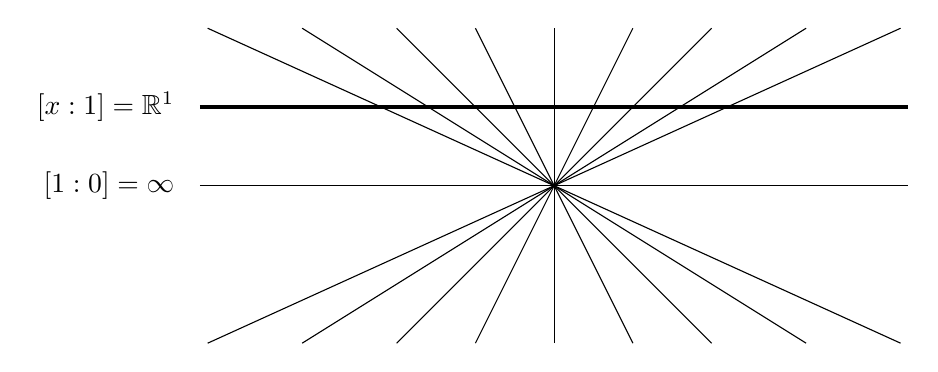
\begin{tikzpicture}
		\draw[very thick] (-4.5,1) -- (4.5,1) ;
		\draw (-4.5,0) -- (4.5,0) ;
		\draw (0,-2) -- (0,2);
		\draw (-2,-2) -- (2,2);
		\draw (-3.2,-2) -- (3.2,2);
		\draw (-1,-2) -- (1,2);
		\draw (2,-2) -- (-2,2);
		\draw (3.2,-2) -- (-3.2,2);
		\draw (1,-2) -- (-1,2);
		\draw (4.4,2) -- (-4.4,-2);
		\draw (4.4,-2) -- (-4.4,2);
		\draw (-4.7,1) node[left] {$[x:1]=\mathbb{R}^1$};
		\draw (-4.7,0) node[left] {$[1:0]=\infty$};
	\end{tikzpicture}
\end{center}
By introduce the continuous mapping
\begin{align*}
	r:P^1(\mathbb{R}) & \longrightarrow\mathbb{R}^1\cup\{\infty\}, \\
	[x:y]             & \longmapsto \frac{x}{y},
\end{align*}
we can clearly see $P^1(\mathbb{R})\cong S^1$.
$P^1(\mathbb{R})$ can be constructed by identifying the antipodal points of $S^1$.
\begin{center}
	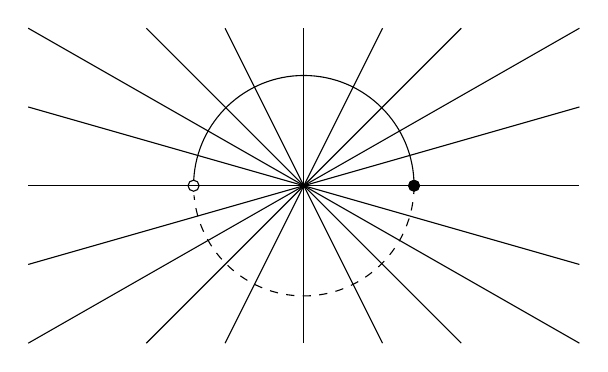
\begin{tikzpicture}
		\draw (1.4,0) arc [start angle=0, end angle=177, radius=1.4cm];
		\draw[dashed] (1.4,0) arc [start angle=0, end angle=-175, radius=1.4cm];
		\draw (-3.5,0) -- (3.5,0) ;
		\draw (0,-2) -- (0,2);
		\draw (-2,-2) -- (2,2);
		\draw (-3.5,-2) -- (3.5,2);
		\draw (-1,-2) -- (1,2);
		\draw (2,-2) -- (-2,2);
		\draw (3.5,-2) -- (-3.5,2);
		\draw (1,-2) -- (-1,2);
		\draw (3.5,1) -- (-3.5,-1);
		\draw (3.5,-1) -- (-3.5,1);
		\draw (-1.4,0) circle [radius=2pt];
		\filldraw (1.4,0) circle [radius=2pt];
	\end{tikzpicture}
\end{center}

\section{Two-dimensional manifolds: examples}
\subsection{Real affine plane $\mathbb{R}^2$}
The real affine plane $\mathbb{R}^2$ carries a standard topology. $\mathbb{R}^2$ is homeomorphic to any open region $G\in\mathbb{R}$.
Since the mapping $(x,y)\mapsto x+\mathrm{i}y$ is a homeomorphism, we have $\mathbb{R}^2\cong \mathbb{C}$.

\subsection{Sphere $S^2$}
The circle $S^2$ is defined by $S^2=\{(x,y,z)\in\mathbb{R}^3|x^2+y^2+z^2=1\}$. Similarly we have $S^2\cong \mathbb{R}^2\cup\{\infty\}$ and the stereographic projection of $P=(0,0,1)$
\begin{align*}
	pr:S^2-P\longrightarrow \mathbb{R}^2,\qquad      & (x, y,z) \longmapsto (X,Y)=\left(\frac{x}{1-z}, \frac{y}{1-z}\right),                                                             \\
	pr^{-1}:\mathbb{R}^1\longrightarrow S^1-P,\qquad & (X,Y) \longmapsto(x, y,z)=\left(\frac{2 X}{X^{2}+Y^{2}+1}, \frac{2 Y}{X^{2}+Y^{2}+1}, \frac{X^{2}+Y^{2}-1}{X^{2}+Y^{2}+1}\right).
\end{align*}
Sphere $S^2$ can be described by a square with some edges identified as follows
\begin{center}
	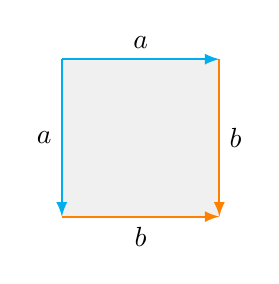
\begin{tikzpicture}
		\fill[fill=gray!12] (-1,-1) --(1,-1)--(1,1)--(-1,1)-- cycle;
		\draw [color=orange,thick,-latex] (-1,-1) -- node [color=black,pos=0.5,below]{$b$} (1,-1);
		\draw [color=cyan,thick,-latex] (-1,1) -- node [color=black,pos=0.5,left]{$a$} (-1,-1);
		\draw [color=orange,thick,-latex] (1,1)--node [color=black,pos=0.5,right]{$b$}(1,-1);
		\draw [color=cyan,thick,-latex] (-1,1)-- node [color=black,pos=0.5,above]{$a$} (1,1);
	\end{tikzpicture}
\end{center}

\subsection{Real projective plane $P^2(\mathbb{R})$}
Real projective plane $P^2(\mathbb{R})=(\mathbb{R}^3-\{(0,0,0)\})/\sim$ where $x\sim y$ whenever there is a nonzero real number $\lambda$ such that $x = \lambda y$. $P^2(\mathbb{R})\cong\mathbb{R}^2\sqcup P^1(\mathbb{R})\cong\mathbb{R}^2\sqcup\mathbb{R}^1\sqcup\{\infty\}$.
\begin{center}
	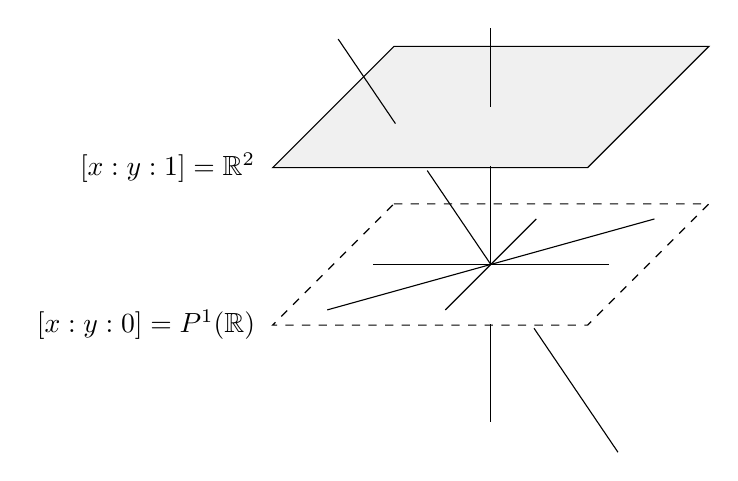
\begin{tikzpicture}
		\draw[dashed] (-2,0,-2) -- (2,0,-2)-- (2,0,2)-- (-2,0,2)--(-2,0,-2);
		\filldraw[fill=gray!12] (-2,2,-2) -- (2,2,-2)-- (2,2,2)-- (-2,2,2)--(-2,2,-2);
		\draw  (1.5,0,-1.5)-- (-1.5,0,1.5);
		\draw  (0,0,-1.5)-- (0,0,1.5);
		\draw  (1.5,0,0)-- (-1.5,0,0);
		\draw (0,-2,0) -- (0,-0.75,0);
		\draw (0,0,0) -- (0,1.25,0);
		\draw (0,2,0) -- (0,3,0);
		\draw (2,-2,1) -- (0.68,-0.68,0.34);
		\draw (0,0,0) -- (-1,1,-0.5);
		\draw (-1.5,1.5,-0.75) -- (-2.4,2.4,-1.2);
		\draw (-2.1,0,2) node[left]{$[x:y:0]=P^1(\mathbb{R})$};
		\draw (-2.1,2,2) node[left]{$[x:y:1]=\mathbb{R}^2$};
	\end{tikzpicture}
\end{center}
$P^2(\mathbb{R})$ can be constructed by identifying the antipodal points of $S^2$, which can be represented by $S^2/\{1,-1\}$. $P^2(\mathbb{R})$ can also be constructed from a closed unit disk $\overline{D^2}$ by identifying the antipodal points of the boundary $\partial \overline{D^2}=S^1$. Another way to describe $P^2(\mathbb{R})$ is a square with some edges identified as follows
\begin{center}
	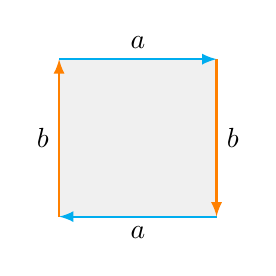
\begin{tikzpicture}
		\fill[fill=gray!12] (-1,-1) --(1,-1)--(1,1)--(-1,1)-- cycle;
		\draw [color=cyan,thick,-latex]  (1,-1)-- node [color=black,pos=0.5,below]{$a$} (-1,-1);
		\draw [color=orange,thick,-latex](-1,-1) -- node [color=black,pos=0.5,left]{$b$} (-1,1) ;
		\draw [color=orange,thick,-latex] (1,1)--node [color=black,pos=0.5,right]{$b$}(1,-1);
		\draw [color=cyan,thick,-latex] (-1,1)-- node [color=black,pos=0.5,above]{$a$} (1,1);
	\end{tikzpicture}
\end{center}
\subsection{Complex projective line $P^1(\mathbb{C})$}
Complex projective line $P^1(\mathbb{C})$ is the set of equivalence classes of $\mathbb{C}^2-{(0,0)}$ under the equivalence relation $\sim$ defined by $x\sim y$ if there is a nonzero complex number $\lambda$ such that $x = \lambda y$. We have the following homeomorphisms $P^1(\mathbb{C})\cong \mathbb{C}\cup\{\infty\}\cong \mathbb{R}^2\cup\{\infty\}\cong S^2$.
\subsection{Torus $T^2$}
A torus $T^2$ is a closed surface defined as the product of two circles $S^1 \times S^1$.
Torus can be described by a square with some edges identified as follows
\begin{center}
	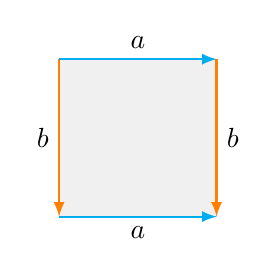
\begin{tikzpicture}
		\fill[fill=gray!12] (-1,-1) --(1,-1)--(1,1)--(-1,1)-- cycle;
		\draw [color=cyan,thick,-latex] (-1,-1) -- node [color=black,pos=0.5,below]{$a$} (1,-1);
		\draw [color=orange,thick,-latex] (-1,1)-- node [color=black,pos=0.5,left]{$b$}(-1,-1)  ;
		\draw [color=orange,thick,-latex] (1,1)--node [color=black,pos=0.5,right]{$b$}(1,-1);
		\draw [color=cyan,thick,-latex] (-1,1)-- node [color=black,pos=0.5,above]{$a$} (1,1);
	\end{tikzpicture}
\end{center}
\subsection{Möbius strip}
Möbius strip can be described by a square with some edges identified as follows
\begin{center}
	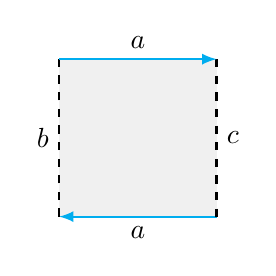
\begin{tikzpicture}
		\fill[fill=gray!12] (-1,-1) --(1,-1)--(1,1)--(-1,1)-- cycle;
		\draw [color=cyan,thick,-latex] (1,-1) -- node [color=black,pos=0.5,below]{$a$} (-1,-1);
		\draw [color=black,thick,dashed](-1,-1) -- node [color=black,pos=0.5,left]{$b$} (-1,1) ;
		\draw [color=black,thick,dashed] (1,1)--node [color=black,pos=0.5,right]{$c$}(1,-1);
		\draw [color=cyan,thick,-latex] (-1,1)-- node [color=black,pos=0.5,above]{$a$} (1,1);
	\end{tikzpicture}
\end{center}
\subsection{Klein bottle}

Klein bottle can be described by a square with some edges identified as follows
\begin{center}
	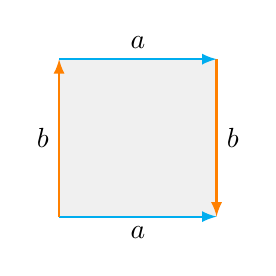
\begin{tikzpicture}
		\fill[fill=gray!12] (-1,-1) --(1,-1)--(1,1)--(-1,1)-- cycle;
		\draw [color=cyan,thick,-latex] (-1,-1) -- node [color=black,pos=0.5,below]{$a$} (1,-1);
		\draw [color=orange,thick,-latex](-1,-1) -- node [color=black,pos=0.5,left]{$b$} (-1,1) ;
		\draw [color=orange,thick,-latex] (1,1)--node [color=black,pos=0.5,right]{$b$}(1,-1);
		\draw [color=cyan,thick,-latex] (-1,1)-- node [color=black,pos=0.5,above]{$a$} (1,1);
	\end{tikzpicture}
\end{center}
\section{Compact two-dimensional manifolds: classification}
\subsection{Orientable surfaces}
Orientable surface of genus $g$ is a surface that has $g$ holes. It is denoted by $M_g$. For $g\ge 1$, $M_g$ can be described by a $4g$-gon with some edges identified as follows
\begin{center}
	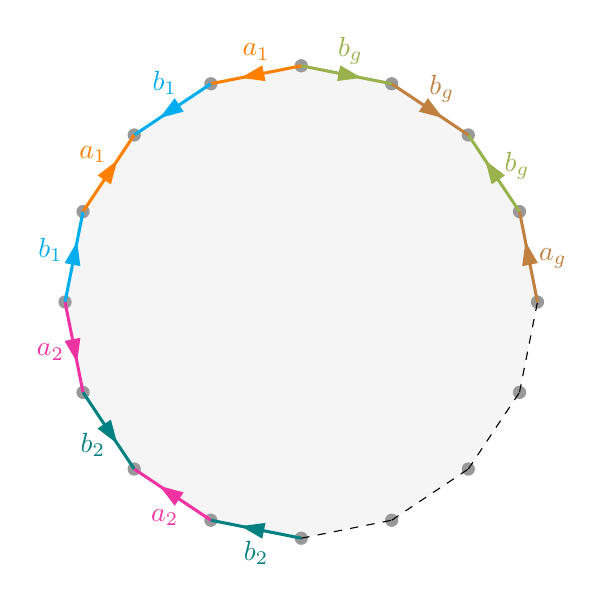
\begin{tikzpicture}
		\def\n{16} % Number of sides
		\def\radius{3cm} % Radius of the circumscribed circle
		\pgfmathsetmacro\startAngle{90} % Starting angle (top point)
	  
		% Define the vertices
		\foreach \i in {1,...,\n} {
		  \pgfmathsetmacro\angle{\startAngle + 360/\n * (\i - 1)}
		  \coordinate (V\i) at (\angle:\radius);
		}
		% Fill the interior region
		\fill[gray!8] (V1)
		\foreach \i in {2,...,\n} {
			-- (V\i)
		} -- cycle;
		\foreach \i in {1,...,\n} {
		  % Plot the vertices
		  \fill[black!40] (V\i) circle (2.4pt);
		}

		  % Draw the edges with arrowheads
		  \draw[->-, line width=1.1pt, color=orange] (V1) -- (V2) node[shift={(0, 0.05)}, midway, above] {$a_1$};
		  \draw[->-, line width=1.1pt, color=cyan] (V2) -- (V3) node[shift={(-0.1, 0.05)}, midway, above] {$b_1$};
		  \draw[-<-, line width=1.1pt, color=orange] (V3) -- (V4) node[shift={(-0.2, 0)}, midway, above] {$a_1$};
		  \draw[-<-, line width=1.1pt, color=cyan] (V4) -- (V5) node[shift={(-0.3, -0.2)}, midway, above] {$b_1$};
		  \draw[->-, line width=1.1pt, color=magenta!80] (V5) -- (V6) node[shift={(-0.3, -0.3)}, midway, above] {$a_2$};
		  \draw[->-, line width=1.1pt, color=teal] (V6) -- (V7) node[shift={(-0.2, 0.1)}, midway, below] {$b_2$};
		  \draw[-<-, line width=1.1pt, color=magenta!80] (V7) -- (V8) node[shift={(-0.1, -0.05)}, midway, below] {$a_2$};
		  \draw[-<-, line width=1.1pt, color=teal] (V8) -- (V9) node[shift={(0, -0.02)}, midway, below] {$b_2$};
		  \draw[dashed] (V9) -- (V10);
		  \draw[dashed] (V10) -- (V11);
		  \draw[dashed] (V11) -- (V12);
		  \draw[dashed] (V12) -- (V13);
		  \draw[->-, line width=1.1pt, color=brown] (V13) -- (V14) node[shift={(0, -0.02)}, midway, right] {$a_g$};
		  \draw[->-, line width=1.1pt, color=lime!40!gray] (V14) -- (V15) node[shift={(0, 0.1)}, midway, right] {$b_g$};
		  \draw[-<-, line width=1.1pt, color=brown] (V15) -- (V16) node[shift={(0.15, -0.05)}, midway, above] {$b_g$};
		  \draw[-<-, line width=1.1pt, color=lime!40!gray] (V16) -- (V1) node[shift={(0.05, 0)}, midway, above] {$b_g$};
	  \end{tikzpicture}
\end{center}
The fundamental group of $M_g$ is given by
\begin{equation*}
	\pi_1(M_g)=\langle a_1,b_1,\dots,a_g,b_g\mid [a_1,b_1]\dots[a_g,b_g]=1\rangle,
\end{equation*}
where $[a,b]=aba^{-1}b^{-1}$ is the commutator of $a$ and $b$. 

The cellular chain complex of $M_g$ is given by
\begin{equation*}
	0\longrightarrow \mathbb{Z} \overset{d_1}{\longrightarrow} \mathbb{Z}^{\oplus 2g}\overset{d_0}{\longrightarrow} \mathbb{Z}\longrightarrow 0,
\end{equation*}
\subsection{Non-orientable surfaces}
Non-orientable surface of genus $g$ is a surface that has  $g$ cross-caps attached to a sphere. It is denoted by $N_g$. For $g\ge 1$, $N_g$ can be described by a $2g$-gon with some edges identified as follows
\begin{center}
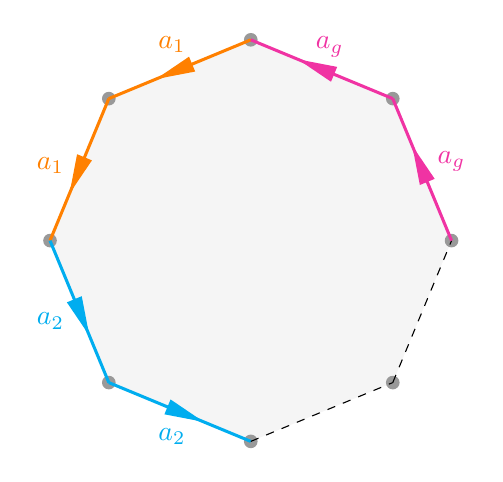
\begin{tikzpicture}[scale=0.85]
	\def\n{8} % Number of sides
	\def\radius{3cm} % Radius of the circumscribed circle
	\pgfmathsetmacro\startAngle{90} % Starting angle (top point)
  
	% Draw the vertices
	\foreach \i in {1,...,\n} {
	  \pgfmathsetmacro\angle{\startAngle + 360/\n * (\i - 1)}
	  \coordinate (V\i) at (\angle:\radius);
	}
	\fill[gray!8] (V1)
		\foreach \i in {2,...,\n} {
			-- (V\i)
		} -- cycle;
	\foreach \i in {1,...,\n} {
	  \fill[black!40] (V\i) circle (2.9pt);
	}
  
	% Draw the edges with arrowheads
	\draw[->-={5mm}, line width=1.1pt, color=orange] (V1) -- (V2) node[shift={(-0.1, 0.07)}, midway, above] {$a_1$};
	\draw[->-={5mm}, line width=1.1pt, color=orange] (V2) -- (V3) node[shift={(-0.06, 0.05)}, midway, left] {$a_1$};
	\draw[->-={5mm}, line width=1.1pt, color=cyan] (V3) -- (V4) node[shift={(-0.06, -0.12)}, midway, left] {$a_2$};
	\draw[->-={5mm}, line width=1.1pt, color=cyan] (V4) -- (V5) node[shift={(-0.1, -0.07)}, midway, below] {$a_2$};
	\draw[dashed] (V5) -- (V6);
	\draw[dashed] (V6) -- (V7);
	\draw[->-={5mm}, line width=1.1pt, color=magenta!80] (V7) -- (V8) node[shift={(0.06, 0.1)}, midway, right] {$a_g$};
	\draw[->-={5mm}, line width=1.1pt, color=magenta!80] (V8) -- (V1) node[shift={(0.1, 0.02)}, midway, above] {$a_g$};
  \end{tikzpicture}
\end{center}
\section{Other manifolds}
\subsection{Real projective space $P^n(\mathbb{R})$}
Real projective plane $P^n(\mathbb{R})=(\mathbb{R}^{n+1}-\{\mathbf{0}\})/\sim$ where $x\sim y$ whenever there is a nonzero real number $\lambda$ such that $x = \lambda y$. In general, we have
$$
	P^n(\mathbb{R})\cong S^n/\{\pm 1\}\cong D^n\sqcup (\partial D^n/{\pm 1})= D^n\sqcup (S^{n-1}/\{\pm 1\})\cong D^n\sqcup P^{n-1}(\mathbb{R})\cong \overline{D^n}\sqcup_{\partial D^n} P^{n-1}(\mathbb{R}),
$$
where $D^n:=\{x\in\mathbb{R}^{n+1}:\Vert x\Vert\le1\}$.

\chapter*{Appendix}

\begin{table}[h]
	\centering
	\begin{tblr}{
		colspec={|Q[m,c,1cm]|Q[m,c,1cm]|Q[m,c,1cm]|Q[m,c,0.8cm]|},
		row{1, 5} = {8ex},
		cell{1, 3, 5}{4} = {green7}}
		\hline
		\SetCell[r=5]{m} $\overline{A}$ & $A^\circ$                     & \SetCell[r=4]{m} $A'$ &\\ \cline{2-2} \cline{4-4}
		                                & \SetCell[r=4]{m} $\partial A$ &                       &\\ \cline{4-4}
		                                &                               &                       &\\ \cline{4-4}
		                                &                               &                       &\\ \cline{3-4}
		                                &                               & $A^s$                 &\\
		\hline
	\end{tblr}
\end{table}
\end{document}
